% !TEX program = xelatex
% 이 파일이 교재 본문의 기준 원본이다.
% 이 폴더에서 xelatex 00.legacy_hdl.tex를 두 번 실행한다.
\documentclass[aspectratio=169,11pt]{beamer}

\usepackage{fontspec}
\usepackage{kotex}
\usepackage{graphicx}
\usepackage{tikz}
\usetikzlibrary{positioning,arrows.meta,automata,shapes.gates.logic.US}
\usepackage{booktabs}

% D2Coding을 저장소에 함께 넣어, 별도 설치 없이 같은 글꼴로 빌드한다.
\setmainfont{D2Coding-Regular.ttf}[Path=../../assets/fonts/,BoldFont={D2Coding-Bold.ttf},ItalicFont={D2Coding-Regular.ttf},BoldItalicFont={D2Coding-Bold.ttf}]
\setmainhangulfont{D2Coding-Regular.ttf}[Path=../../assets/fonts/,BoldFont={D2Coding-Bold.ttf},ItalicFont={D2Coding-Regular.ttf},BoldItalicFont={D2Coding-Bold.ttf}]
\setsansfont{D2Coding-Regular.ttf}[Path=../../assets/fonts/,BoldFont={D2Coding-Bold.ttf},ItalicFont={D2Coding-Regular.ttf},BoldItalicFont={D2Coding-Bold.ttf}]
\setsanshangulfont{D2Coding-Regular.ttf}[Path=../../assets/fonts/,BoldFont={D2Coding-Bold.ttf},ItalicFont={D2Coding-Regular.ttf},BoldItalicFont={D2Coding-Bold.ttf}]
\setmonofont{D2Coding-Regular.ttf}[Path=../../assets/fonts/,BoldFont={D2Coding-Bold.ttf},ItalicFont={D2Coding-Regular.ttf},BoldItalicFont={D2Coding-Bold.ttf}]

% University of Seoul identity color
\definecolor{UOSBlue}{HTML}{005EB8}
\definecolor{TextGray}{HTML}{303030}

\setbeamertemplate{navigation symbols}{}
\setbeamercolor{normal text}{fg=TextGray,bg=white}
\setbeamercolor{frametitle}{fg=UOSBlue,bg=white}
\setbeamercolor{title}{fg=white}
\setbeamercolor{structure}{fg=UOSBlue}
\setbeamertemplate{itemize item}{\color{UOSBlue}\small$\bullet$}
\setbeamertemplate{itemize subitem}{\color{UOSBlue}\scriptsize$\bullet$}
\setbeamertemplate{frametitle}{%
  \vspace{0.55cm}\hspace{0.48cm}\insertframetitle\par\vspace{0.12cm}}
\setbeamerfont{frametitle}{series=\bfseries,size=\Large}
\setbeamerfont{section in toc}{size=\large,shape=\upshape}
\setbeamerfont{subsection in toc}{size=\normalsize,shape=\upshape}
\setbeamertemplate{section in toc}[sections numbered]
% Beamer 목차 파일의 네 번째 인수는 해당 절의 시작 페이지다.
\makeatletter
\patchcmd{\beamer@subsectionintoc}
  {\def\inserttocsubsectionnumber{#2}}
  {\def\inserttocsubsectionnumber{#2}\def\inserttocsubsectionpage{#4}}
  {}{\PackageError{legacy-hdl}{Cannot add TOC page numbers}{Check Beamer TOC implementation.}}
\makeatother
\setbeamertemplate{subsection in toc}{%
  \leavevmode\leftskip=1em%
  \inserttocsubsection\hfill\inserttocsubsectionpage\par}
\setbeamerfont{subsection in toc}{size=\footnotesize,shape=\upshape}
% 목차와 PDF 북마크는 본문의 subsection에서 함께 생성한다.
\newcommand{\chaptercontents}[2]{%
  \begin{frame}[t]{#2}
    \tableofcontents[sections={#1},sectionstyle=show/show,subsectionstyle=show/show/show]
  \end{frame}}
\setbeamersize{text margin left=0.8cm,text margin right=0.8cm}
\setbeamerfont{itemize/enumerate body}{shape=\upshape}
\setbeamerfont{itemize/enumerate subbody}{shape=\upshape}

% 실제 높이를 예약해 본문과 로고가 겹치지 않게 한다.
\setbeamertemplate{footline}{%
  \leavevmode
  \hbox to \paperwidth{%
    \hspace{0.8cm}\hbox to 0.6cm{}%
    \hfill
    
\includegraphics[width=2.64cm,trim=58bp 385bp 58bp 385bp,clip]{../../assets/uos-logo-horizontal.png}%
    \hfill
    \hbox to 0.6cm{\hfil\color{gray}\scriptsize\insertframenumber}%
    \hspace{0.8cm}}%
  \vspace{0.30cm}}

\newcommand{\week}{FPGA}
\newcommand{\course}{전자전기컴퓨터설계실험Ⅱ}
\newcommand{\topic}{디지털 회로 실험 교재}
\newcommand{\presentationdate}{2026. 09. 07.}

\title{\course\\\week. \topic}
\author{}
\hypersetup{pdfauthor={}}
\date{\presentationdate}


\usepackage{listings}
\lstset{basicstyle=\ttfamily\scriptsize,breaklines=true,columns=fullflexible}
% 세부 원자료 위치는 TeX에만 보존하고, PDF 출처는 마지막 장에서 안내한다.
\newcommand{\sourceref}[1]{}
\newcommand{\captureroot}{../../../example/fpga_projects_hdl/legacy_all_hdl/captures}
% CodeSnap PNG의 원본 줄을 잘라 표시한다. PNG 자체는 변경하지 않는다.
% 인수: 제목, 파일, 아래 여백(bp), 위 여백(bp), 원본 경로, 줄 범위
\newcommand{\codepage}[7]{%
  \begin{frame}[t]{#1 / 코드}
    \if\relax\detokenize{#7}\relax\else\label{#7}\fi
    {\scriptsize\texttt{\detokenize{#5}}\hfill L#6\par}
    \vspace{0.12cm}
    \centering
    \includegraphics[trim=32bp #3bp 32bp #4bp,clip,width=\textwidth,height=5.45cm,keepaspectratio]{\captureroot/#2}
  \end{frame}}
\newcommand{\checkpage}[4]{%
  \begin{frame}[t]{#1 / 시뮬레이션 확인}
    \small
    \begin{block}{확인할 계층}
      \texttt{\detokenize{#2}}
    \end{block}
    \begin{itemize}
      \item #3
      \item #4
      \item 입력을 바꾸기 전에 예상 출력을 적고, VCD의 값과 비교한다.
    \end{itemize}
  \end{frame}}

\begin{document}


% 표지
{\setbeamertemplate{footline}{}
\setbeamercolor{background canvas}{bg=UOSBlue}
\begin{frame}[plain]
  \begin{tikzpicture}[remember picture,overlay]
    \node[anchor=north west,inner sep=0pt,text=white,font=\bfseries\fontsize{27}{33}\selectfont,align=left]
      at ([xshift=1.53cm,yshift=-1.5cm]current page.north west) {\course\\\week. \topic};
    \node[anchor=south west,inner sep=0pt] at ([xshift=1.38cm,yshift=0.98cm]current page.south west)
      {
\includegraphics[width=1.45cm]{../../assets/uos-logo-white.png}};
    \node[anchor=south east,text=white,font=\small\bfseries,align=right]
      at ([xshift=-1.38cm,yshift=0.98cm]current page.south east)
      {기존 강의자료 기반 재구성\\\presentationdate};
  \end{tikzpicture}
\end{frame}}


\chaptercontents{1}{목차 1/7 | 조합회로}
\chaptercontents{2}{목차 2/7 | 순차회로}
\chaptercontents{3}{목차 3/7 | 표시 장치}
\chaptercontents{4}{목차 4/7 | 파형 생성과 구동}
\chaptercontents{5}{목차 5/7 | 상태 머신}
\chaptercontents{6}{목차 6/7 | 인터페이스와 통합 검증}
\chaptercontents{7}{목차 7/7 | 출처와 보충 자료}
\begin{frame}{교재와 프로젝트의 범위}
\begin{itemize}
\item 2022년 교안의 30개 번호 실습, 첫 카운터, 상태 머신 응용을 주제별로 재작성했다.
\item 프로젝트 생성과 합성 절차의 반복 화면은 제외했다.
\item 새 코드는 37개 설계 모듈과 테스트벤치 하나다. 6개 계층에서 33개 실습·보충 항목을 검증한다.
\item 구형 보드 핀맵과 시뮬레이션용 입출력을 구분한다. 보드 연결 전 XDC를 대조한다.
\end{itemize}
\end{frame}
\begin{frame}{하나의 프로젝트, 여섯 개 계층}
\begin{itemize}
\item \texttt{tb\_legacy / dut / u\_comb}: 게이트·선택·산술
\item \texttt{u\_seq}: 카운터·저장·시프트
\item \texttt{u\_display}: BCD·7세그먼트·LCD 명령
\item \texttt{u\_waveform}: PWM·음원·모터 위상
\item \texttt{u\_fsm}: Moore·Mealy·상태 전이
\item \texttt{u\_interface}: UART 송수신 루프백
\end{itemize}
\end{frame}
\begin{frame}{분기와 반복을 회로로 표현하기}
\begin{itemize}
\item 조합회로의 \texttt{if/case}는 입력에 따라 결과를 선택하는 회로를 표현한다.
\item 클록마다 상태를 갱신하면 시간에 따른 반복 동작을 만든다.
\item 합성 가능한 고정 횟수 \texttt{for}는 반복되는 하드웨어를 기술할 수 있다.
\item 테스트벤치의 반복문은 입력을 바꾸며 회로를 검사한다. 같은 문법도 역할이 다르다.
\end{itemize}
\end{frame}
\begin{frame}{원자료를 읽을 때의 주의점}
\begin{itemize}
\item 원자료의 \texttt{LVCMOSS33} 표기는 오타다. XDC의 실제 속성값은 \texttt{LVCMOS33}이다.
\item 표시된 핀 번호는 그 페이지의 원본 예제에 해당한다. 새 탑모듈의 포트에 그대로 복사하지 않는다.
\item 클록을 버튼으로 직접 공급하는 과거 예제와 단일 기준 클록으로 동작하는 새 코드를 구분한다.
\item 원본과 새 코드의 비트 순서·폭·상태 동작이 다르면 각 실습에서 차이를 밝힌다.
\end{itemize}
\end{frame}
\section{조합회로}
\chaptercontents{1}{조합회로 / 구성}
\subsection{실습 1 / AND, OR, XOR 게이트 구현}
\begin{frame}[t]{실습 1 / AND, OR, XOR 게이트 구현}
\small
\begin{columns}[T,onlytextwidth]\begin{column}{0.47\textwidth}\begin{center}\renewcommand{\arraystretch}{1.12}\begin{tabular}{ccccc}\hline a & b & AND & OR & XOR\\\hline 0 & 0 & 0 & 0 & 0\\
0 & 1 & 0 & 1 & 1\\
1 & 0 & 0 & 1 & 1\\
1 & 1 & 1 & 1 & 0\\\hline\end{tabular}\end{center}\end{column}\begin{column}{0.49\textwidth}\begin{itemize}\setlength{\itemsep}{0.5em}\item AND는 모두 1, OR는 하나 이상 1, XOR는 입력이 다를 때 1이다.
\item 비트 연산자는 \texttt{\&}, \texttt{|}, \texttt{\^{}}다. 논리 연산자와 구분한다.
\item 입력 4가지 조합을 모두 검사한다. 조합회로이므로 클록은 필요하지 않다.\end{itemize}\end{column}\end{columns}
\sourceref{2.2\_논리 게이트 구현, p.4}
\end{frame}
\begin{frame}[t]{실습 1 / 핀 참고}
\fontsize{8}{9}\selectfont
원래 예제의 포트 이름과 패키지 핀. 새 시뮬레이션 탑에는 적용하지 않는다.
\begin{center}\renewcommand{\arraystretch}{1.0}
\begin{tabular}{ll@{\hspace{1.1cm}}ll}\toprule
포트 & 핀 & 포트 & 핀\\\midrule
\texttt{a} & K4 & \texttt{y} & M4 \\
\texttt{x} & L4 & \texttt{z} & M2 \\
\texttt{b} & N8 & \texttt{} &  \\\bottomrule\end{tabular}\end{center}
{\scriptsize \par}
\sourceref{2.2\_논리 게이트 구현, p.24}\end{frame}

\checkpage{실습 1 / AND, OR, XOR 게이트}{tb_legacy.dut.u_comb.u_gates}{a,b에 00, 01, 10, 11을 넣는다.}{and\_out, or\_out, xor\_out을 진리표의 같은 행과 비교한다.}
\codepage{실습 1 / AND, OR, XOR 게이트}{codesnap/src__combinational__logic_gates__01.png}{440}{166}{src/combinational/logic_gates.v}{1-12}{code:src/combinational/logic_gates.v}
\codepage{실습 1 / AND, OR, XOR 게이트}{codesnap/src__combinational__logic_gates__01.png}{76}{790}{src/combinational/logic_gates.v}{13-19}{}
\subsection{실습 2 / NOT 게이트 구현}
\begin{frame}[t]{실습 2 / NOT 게이트 구현}
\small
\begin{columns}[T,onlytextwidth]\begin{column}{0.47\textwidth}\begin{center}\renewcommand{\arraystretch}{1.12}\begin{tabular}{cc}\hline a & z\\\hline 0 & 1\\
1 & 0\\\hline\end{tabular}\end{center}\end{column}\begin{column}{0.49\textwidth}\begin{itemize}\setlength{\itemsep}{0.5em}\item 비트 반전은 \texttt{\textasciitilde a}. 0과 1을 서로 바꾼다.
\item 버스 반전은 모든 비트에 적용된다. 논리 부정 !는 입력 전체가 0인지 판정한다.
\item 입력이 바뀌면 조합 논리를 거쳐 출력에 반영된다.\end{itemize}\end{column}\end{columns}
\sourceref{2.2\_논리 게이트 구현, p.54}
\end{frame}
\begin{frame}[t]{실습 2 / 핀 참고}
\fontsize{8}{9}\selectfont
원래 예제의 포트 이름과 패키지 핀. 새 시뮬레이션 탑에는 적용하지 않는다.
\begin{center}\renewcommand{\arraystretch}{1.0}
\begin{tabular}{ll@{\hspace{1.1cm}}ll}\toprule
포트 & 핀 & 포트 & 핀\\\midrule
\texttt{a} & K4 & \texttt{z} & L4 \\\bottomrule\end{tabular}\end{center}
{\scriptsize \par}
\sourceref{2.2\_논리 게이트 구현, p.71}\end{frame}

\checkpage{실습 2 / NOT 게이트}{tb_legacy.dut.u_comb.u_gates}{a에 0과 1을 번갈아 넣는다.}{not\_out은 각각 1과 0이다. 클록을 기다리는 회로가 아니다.}
\begin{frame}{실습 2 / NOT 게이트 / 코드 연결}
\small\texttt{\detokenize{src/combinational/logic_gates.v}}\\[0.4cm]
전체 코드는 p.~\pageref{code:src/combinational/logic_gates.v}부터 수록했다.\\[0.3cm]
이 실습의 입력·출력은 앞의 확인 항목과 함께 읽는다.
\end{frame}
\subsection{실습 3 / 전가산기 구현}
\begin{frame}[t]{실습 3 / 전가산기 구현}
\small
\begin{columns}[T,onlytextwidth]\begin{column}{0.47\textwidth}\begin{center}\renewcommand{\arraystretch}{1.12}\begin{tabular}{ccccc}\hline a & b & cin & sum & cout\\\hline 0 & 0 & 0 & 0 & 0\\
0 & 0 & 1 & 1 & 0\\
0 & 1 & 0 & 1 & 0\\
0 & 1 & 1 & 0 & 1\\
1 & 0 & 0 & 1 & 0\\
1 & 0 & 1 & 0 & 1\\
1 & 1 & 0 & 0 & 1\\
1 & 1 & 1 & 1 & 1\\\hline\end{tabular}\end{center}\end{column}\begin{column}{0.49\textwidth}\begin{itemize}\setlength{\itemsep}{0.5em}\item $sum=a\oplus b\oplus cin$. 입력 세 비트의 합을 두 비트로 표현한다.
\item $cout=ab+(a\oplus b)cin$. 반가산기 두 개와 OR로 구성한다.
\item 새 full\_adder는 half\_adder 두 개를 연결한 계층 구조다.\end{itemize}\end{column}\end{columns}
\sourceref{2.2\_논리 게이트 구현, p.94, 95}
\end{frame}

\begin{frame}[t]{실습 3 / 핀 참고}
\fontsize{8}{9}\selectfont
원래 예제의 포트 이름과 패키지 핀. 새 시뮬레이션 탑에는 적용하지 않는다.
\begin{center}\renewcommand{\arraystretch}{1.0}
\begin{tabular}{ll@{\hspace{1.1cm}}ll}\toprule
포트 & 핀 & 포트 & 핀\\\midrule
\texttt{a} & K4 & \texttt{cout} & M4 \\
\texttt{s} & L4 & \texttt{cin} & N4 \\
\texttt{b} & N8 & \texttt{} &  \\\bottomrule\end{tabular}\end{center}
{\scriptsize \par}
\sourceref{2.2\_논리 게이트 구현, p.111}\end{frame}

\checkpage{실습 3 / 전가산기}{tb_legacy.dut.u_comb.u_bit1}{a,b,carry\_in의 8가지 조합을 모두 검사한다.}{\{carry\_out,sum\}은 세 입력의 합이다. 1+1+1의 결과는 11이다.}
\codepage{실습 3 / 전가산기}{codesnap/src__combinational__full_adder__01.png}{1064}{166}{src/combinational/full_adder.v}{1-12}{code:src/combinational/full_adder.v}
\codepage{실습 3 / 전가산기}{codesnap/src__combinational__full_adder__01.png}{440}{790}{src/combinational/full_adder.v}{13-24}{}
\codepage{실습 3 / 전가산기}{codesnap/src__combinational__full_adder__01.png}{76}{1414}{src/combinational/full_adder.v}{25-31}{}
\subsection{실습 4 / 전감산기 구현}
\begin{frame}[t]{실습 4 / 전감산기 구현}
\small
\begin{columns}[T,onlytextwidth]\begin{column}{0.47\textwidth}\begin{center}\renewcommand{\arraystretch}{1.12}\begin{tabular}{ccccc}\hline a & b & bin & diff & borrow\\\hline 0 & 0 & 0 & 0 & 0\\
0 & 0 & 1 & 1 & 1\\
0 & 1 & 0 & 1 & 1\\
0 & 1 & 1 & 0 & 1\\
1 & 0 & 0 & 1 & 0\\
1 & 0 & 1 & 0 & 0\\
1 & 1 & 0 & 0 & 0\\
1 & 1 & 1 & 1 & 1\\\hline\end{tabular}\end{center}\end{column}\begin{column}{0.49\textwidth}\begin{itemize}\setlength{\itemsep}{0.5em}\item $diff=a\oplus b\oplus bin$. 자리빌림 입력까지 빼는 회로다.
\item $borrow=(\overline a b)+(\overline{a\oplus b}\,bin)$.
\item 0−1−1=−2는 diff=0, borrow=1이다. 원자료 c/cin은 bin으로 통일한다.\end{itemize}\end{column}\end{columns}
\sourceref{2.2\_논리 게이트 구현, p.133, 134}
\end{frame}

\begin{frame}[t]{실습 4 / 핀 참고}
\fontsize{8}{9}\selectfont
원래 예제의 포트 이름과 패키지 핀. 새 시뮬레이션 탑에는 적용하지 않는다.
\begin{center}\renewcommand{\arraystretch}{1.0}
\begin{tabular}{ll@{\hspace{1.1cm}}ll}\toprule
포트 & 핀 & 포트 & 핀\\\midrule
\texttt{a} & K4 & \texttt{bor} & M4 \\
\texttt{d} & L4 & \texttt{cin} & N4 \\
\texttt{b} & N8 & \texttt{} &  \\\bottomrule\end{tabular}\end{center}
{\scriptsize \par}
\sourceref{2.2\_논리 게이트 구현, p.149}\end{frame}

\checkpage{실습 4 / 전감산기}{tb_legacy.dut.u_comb.u_subtractor}{a,b,borrow\_in의 8가지 조합을 넣는다.}{0-1-1에서 difference=0, borrow\_out=1인지 확인한다.}
\codepage{실습 4 / 전감산기}{codesnap/src__combinational__full_subtractor__01.png}{284}{166}{src/combinational/full_subtractor.v}{1-12}{code:src/combinational/full_subtractor.v}
\codepage{실습 4 / 전감산기}{codesnap/src__combinational__full_subtractor__01.png}{76}{790}{src/combinational/full_subtractor.v}{13-16}{}
\subsection{실습 5 / 8X3 ENCODER 설계}
\begin{frame}[t]{실습 5 / 8X3 ENCODER 설계}
\small
\begin{columns}[T,onlytextwidth]\begin{column}{0.47\textwidth}\begin{center}\renewcommand{\arraystretch}{1.12}\begin{tabular}{cc}\hline i[7:0] & a[2:0]\\\hline 10000000 & 000\\
01000000 & 001\\
00100000 & 010\\
00010000 & 011\\
00001000 & 100\\
00000100 & 101\\
00000010 & 110\\
00000001 & 111\\\hline\end{tabular}\end{center}\end{column}\begin{column}{0.49\textwidth}\begin{itemize}\setlength{\itemsep}{0.5em}\item 원자료는 MSB 쪽 입력을 0번으로 부호화한다. 비트 번호를 그대로 출력하는 방식과 다르다.
\item 한 비트만 1인 one-hot 입력을 전제로 한다.
\item 입력이 0이거나 여러 비트가 1이면 valid=0이다. 우선순위 인코더와 구분한다.\end{itemize}\end{column}\end{columns}
\sourceref{3.1\_기초 조합 논리 회로 설계, p.4, 5}
\end{frame}

\begin{frame}[t]{실습 5 / 핀 참고}
\fontsize{8}{9}\selectfont
원래 예제의 포트 이름과 패키지 핀. 새 시뮬레이션 탑에는 적용하지 않는다.
\begin{center}\renewcommand{\arraystretch}{1.0}
\begin{tabular}{ll@{\hspace{1.1cm}}ll}\toprule
포트 & 핀 & 포트 & 핀\\\midrule
\texttt{i[7]} & K4 & \texttt{a[2]} & L4 \\
\texttt{i[1]} & L5 & \texttt{i[3]} & P6 \\
\texttt{i[6]} & N8 & \texttt{a[1]} & M4 \\
\texttt{i[0]} & J2 & \texttt{i[2]} & N6 \\
\texttt{i[5]} & N4 & \texttt{a[0]} & M2 \\
\texttt{i[4]} & N1 & \texttt{} &  \\\bottomrule\end{tabular}\end{center}
{\scriptsize \par}
\sourceref{3.1\_기초 조합 논리 회로 설계, p.19}\end{frame}

\checkpage{실습 5 / 8X3 ENCODER}{tb_legacy.dut.u_comb.u_encoder}{one\_hot=10000000이면 code=0, 00000001이면 code=7이다.}{모두 0 또는 여러 비트가 1이면 valid=0이다. code만 보고 유효성을 판단하지 않는다.}
\codepage{실습 5 / 8X3 ENCODER}{codesnap/src__combinational__encoder8to3__01.png}{960}{166}{src/combinational/encoder8to3.v}{1-12}{code:src/combinational/encoder8to3.v}
\codepage{실습 5 / 8X3 ENCODER}{codesnap/src__combinational__encoder8to3__01.png}{336}{790}{src/combinational/encoder8to3.v}{13-24}{}
\codepage{실습 5 / 8X3 ENCODER}{codesnap/src__combinational__encoder8to3__01.png}{76}{1414}{src/combinational/encoder8to3.v}{25-29}{}
\subsection{실습 6 / 3X8 DECODER 설계}
\begin{frame}[t]{실습 6 / 3X8 DECODER 설계}
\small
\begin{columns}[T,onlytextwidth]\begin{column}{0.47\textwidth}\begin{center}\renewcommand{\arraystretch}{1.12}\begin{tabular}{cc}\hline abc & o[7:0]\\\hline 000 & 00000001\\
001 & 00000010\\
010 & 00000100\\
011 & 00001000\\
100 & 00010000\\
101 & 00100000\\
110 & 01000000\\
111 & 10000000\\\hline\end{tabular}\end{center}\end{column}\begin{column}{0.49\textwidth}\begin{itemize}\setlength{\itemsep}{0.5em}\item 3비트 입력으로 8개 출력 중 하나를 선택한다. 000은 o[0]을 켠다.
\item 새 코드: \texttt{8'b0000\_0001 << select}. 결과 폭은 8비트다.
\item 앞 인코더의 MSB-first 규칙과 반대이므로 단순 직결하면 역함수가 되지 않는다.\end{itemize}\end{column}\end{columns}
\sourceref{3.1\_기초 조합 논리 회로 설계, p.41, 42}
\end{frame}

\begin{frame}[t]{실습 6 / 핀 참고}
\fontsize{8}{9}\selectfont
원래 예제의 포트 이름과 패키지 핀. 새 시뮬레이션 탑에는 적용하지 않는다.
\begin{center}\renewcommand{\arraystretch}{1.0}
\begin{tabular}{ll@{\hspace{1.1cm}}ll}\toprule
포트 & 핀 & 포트 & 핀\\\midrule
\texttt{a} & K4 & \texttt{o[2]} & M3 \\
\texttt{o[5]} & M2 & \texttt{o[7]} & L4 \\
\texttt{b} & N8 & \texttt{o[1]} & M1 \\
\texttt{o[4]} & N7 & \texttt{o[6]} & M4 \\
\texttt{c} & N4 & \texttt{o[0]} & N5 \\
\texttt{o[3]} & M7 & \texttt{} &  \\\bottomrule\end{tabular}\end{center}
{\scriptsize \par}
\sourceref{3.1\_기초 조합 논리 회로 설계, p.56}\end{frame}

\checkpage{실습 6 / 3X8 DECODER}{tb_legacy.dut.u_comb}{select를 0부터 7까지 바꾼다.}{decoded는 00000001부터 10000000까지 이동한다. 항상 한 비트만 1이다.}
\codepage{실습 6 / 3X8 DECODER}{codesnap/src__combinational__lab_combinational__01.png}{1064}{166}{src/combinational/lab_combinational.v}{1-12}{code:src/combinational/lab_combinational.v}
\codepage{실습 6 / 3X8 DECODER}{codesnap/src__combinational__lab_combinational__01.png}{440}{790}{src/combinational/lab_combinational.v}{13-24}{}
\codepage{실습 6 / 3X8 DECODER}{codesnap/src__combinational__lab_combinational__01.png}{76}{1414}{src/combinational/lab_combinational.v}{25-31}{}
\codepage{실습 6 / 3X8 DECODER}{codesnap/src__combinational__lab_combinational__02.png}{1012}{166}{src/combinational/lab_combinational.v}{32-43}{}
\codepage{실습 6 / 3X8 DECODER}{codesnap/src__combinational__lab_combinational__02.png}{388}{790}{src/combinational/lab_combinational.v}{44-55}{}
\codepage{실습 6 / 3X8 DECODER}{codesnap/src__combinational__lab_combinational__02.png}{76}{1414}{src/combinational/lab_combinational.v}{56-61}{}
\codepage{실습 6 / 3X8 DECODER}{codesnap/src__combinational__lab_combinational__03.png}{1220}{166}{src/combinational/lab_combinational.v}{62-73}{}
\codepage{실습 6 / 3X8 DECODER}{codesnap/src__combinational__lab_combinational__03.png}{596}{790}{src/combinational/lab_combinational.v}{74-85}{}
\codepage{실습 6 / 3X8 DECODER}{codesnap/src__combinational__lab_combinational__03.png}{76}{1414}{src/combinational/lab_combinational.v}{86-95}{}
\codepage{실습 6 / 3X8 DECODER}{codesnap/src__combinational__lab_combinational__04.png}{76}{166}{src/combinational/lab_combinational.v}{96-104}{}
\subsection{실습 7 / 4BIT MULTIPLEXER 설계}
\begin{frame}[t]{실습 7 / 4BIT MULTIPLEXER 설계}
\small
\begin{columns}[T,onlytextwidth]\begin{column}{0.47\textwidth}\begin{center}\renewcommand{\arraystretch}{1.12}\begin{tabular}{cc}\hline sel[1:0] & z\\\hline 00 & i[3]\\
01 & i[2]\\
10 & i[1]\\
11 & i[0]\\\hline\end{tabular}\end{center}\end{column}\begin{column}{0.49\textwidth}\begin{itemize}\setlength{\itemsep}{0.5em}\item 여러 입력 중 하나를 출력으로 선택한다.
\item 원자료 세 번째 행의 00은 10으로 바로잡았다. MSB-first 순서는 유지한다.
\item \texttt{mux4to1}은 표의 MSB-first 4:1 선택을 구현한다. 별도 \texttt{a[select]}는 보충 8:1 예제다.\end{itemize}\end{column}\end{columns}
\sourceref{3.1\_기초 조합 논리 회로 설계, p.78, 79}
\end{frame}

\begin{frame}[t]{실습 7 / 핀 참고}
\fontsize{8}{9}\selectfont
원래 예제의 포트 이름과 패키지 핀. 새 시뮬레이션 탑에는 적용하지 않는다.
\begin{center}\renewcommand{\arraystretch}{1.0}
\begin{tabular}{ll@{\hspace{1.1cm}}ll}\toprule
포트 & 핀 & 포트 & 핀\\\midrule
\texttt{i[3]} & K4 & \texttt{i[1]} & N4 \\
\texttt{s[1]} & Y1 & \texttt{i[0]} & Y7 \\
\texttt{i[2]} & N8 & \texttt{z} & L4 \\
\texttt{s[0]} & W3 & \texttt{} &  \\\bottomrule\end{tabular}\end{center}
{\scriptsize \par}
\sourceref{3.1\_기초 조합 논리 회로 설계, p.93}\end{frame}

\checkpage{실습 7 / 4BIT MULTIPLEXER}{tb_legacy.dut.u_comb.u_mux4}{data=1010에서 select를 00,01,10,11로 바꾼다.}{selected는 1,0,1,0이다. select=0이 data[3]을 고른다.}
\codepage{실습 7 / 4BIT MULTIPLEXER}{codesnap/src__combinational__mux4to1__01.png}{544}{166}{src/combinational/mux4to1.v}{1-12}{code:src/combinational/mux4to1.v}
\codepage{실습 7 / 4BIT MULTIPLEXER}{codesnap/src__combinational__mux4to1__01.png}{76}{790}{src/combinational/mux4to1.v}{13-21}{}
\subsection{실습 8 / 1X8 DEMULTIPLEXER 설계}
\begin{frame}[t]{실습 8 / 1X8 DEMULTIPLEXER 설계}
\small
\begin{columns}[T,onlytextwidth]\begin{column}{0.47\textwidth}\begin{center}\renewcommand{\arraystretch}{1.12}\begin{tabular}{cc}\hline sel & 입력을 전달할 출력\\\hline 000 & o[7]\\
001 & o[6]\\
010 & o[5]\\
011 & o[4]\\
100 & o[3]\\
101 & o[2]\\
110 & o[1]\\
111 & o[0]\\\hline\end{tabular}\end{center}\end{column}\begin{column}{0.49\textwidth}\begin{itemize}\setlength{\itemsep}{0.5em}\item 입력 i를 선택된 출력으로 보내고 나머지는 0으로 둔다.
\item 원자료는 000일 때 o[7], 111일 때 o[0]을 선택한다.
\item 디코더 출력과 i를 AND한 구조로 해석할 수 있다. i=0이면 모든 출력이 0이다.\end{itemize}\end{column}\end{columns}
\sourceref{3.1\_기초 조합 논리 회로 설계, p.115, 116}
\end{frame}

\begin{frame}[t]{실습 8 / 핀 참고}
\fontsize{8}{9}\selectfont
원래 예제의 포트 이름과 패키지 핀. 새 시뮬레이션 탑에는 적용하지 않는다.
\begin{center}\renewcommand{\arraystretch}{1.0}
\begin{tabular}{ll@{\hspace{1.1cm}}ll}\toprule
포트 & 핀 & 포트 & 핀\\\midrule
\texttt{i} & K4 & \texttt{o[3]} & M7 \\
\texttt{o[6]} & M4 & \texttt{s[0]} & U2 \\
\texttt{o[5]} & M2 & \texttt{o[2]} & M3 \\
\texttt{s[2]} & Y1 & \texttt{o[1]} & M1 \\
\texttt{o[4]} & N7 & \texttt{o[7]} & L4 \\
\texttt{s[1]} & W3 & \texttt{o[0]} & N5 \\\bottomrule\end{tabular}\end{center}
{\scriptsize \par}
\sourceref{3.1\_기초 조합 논리 회로 설계, p.130}\end{frame}

\checkpage{실습 8 / 1X8 DEMULTIPLEXER}{tb_legacy.dut.u_comb.u_demux8}{data=1에서 select를 0부터 7까지 바꾼다.}{routed의 1이 MSB에서 LSB로 이동한다. data=0이면 전체 출력이 0이다.}
\codepage{실습 8 / 1X8 DEMULTIPLEXER}{codesnap/src__combinational__demux1to8__01.png}{128}{166}{src/combinational/demux1to8.v}{1-12}{code:src/combinational/demux1to8.v}
\codepage{실습 8 / 1X8 DEMULTIPLEXER}{codesnap/src__combinational__demux1to8__01.png}{76}{790}{src/combinational/demux1to8.v}{13-13}{}
\subsection{실습 9 / 크기 비교기}
\begin{frame}[t]{실습 9 / 크기 비교기}
\small
\begin{columns}[T,onlytextwidth]\begin{column}{0.47\textwidth}\begin{center}\renewcommand{\arraystretch}{1.12}\begin{tabular}{cc}\hline 조건 & o[2:0]\\\hline A>B & 100\\
A=B & 010\\
A<B & 001\\\hline\end{tabular}\end{center}\end{column}\begin{column}{0.49\textwidth}\begin{itemize}\setlength{\itemsep}{0.5em}\item 두 4비트 unsigned 입력을 비교한다. 세 조건 중 하나만 참이다.
\item 같음은 ==, 대소는 > 또는 <다. =는 비교가 아니라 대입이다.
\item A=0/B=15, A=B, A=15/B=0의 경계를 먼저 확인한다.\end{itemize}\end{column}\end{columns}
\sourceref{4.1\_고급 조합논리 회로 설계, p.4, 5}
\end{frame}

\begin{frame}[t]{실습 9 / 핀 참고}
\fontsize{8}{9}\selectfont
원래 예제의 포트 이름과 패키지 핀. 새 시뮬레이션 탑에는 적용하지 않는다.
\begin{center}\renewcommand{\arraystretch}{1.0}
\begin{tabular}{ll@{\hspace{1.1cm}}ll}\toprule
포트 & 핀 & 포트 & 핀\\\midrule
\texttt{a[3]} & Y1 & \texttt{o[2]} & L4 \\
\texttt{b[1]} & V4 & \texttt{b[3]} & W4 \\
\texttt{a[2]} & W3 & \texttt{o[1]} & M4 \\
\texttt{b[0]} & U4 & \texttt{b[2]} & W1 \\
\texttt{a[1]} & U2 & \texttt{o[0]} & M2 \\
\texttt{a[0]} & T1 & \texttt{} &  \\\bottomrule\end{tabular}\end{center}
{\scriptsize \par}
\sourceref{4.1\_고급 조합논리 회로 설계, p.19}\end{frame}

\checkpage{실습 9 / 크기 비교기}{tb_legacy.dut.u_comb}{a[3:0], b[3:0]에 (0,15), (7,7), (15,0)을 넣는다.}{새 코드에서는 result[27]이 A>B, result[28]이 A=B다. 원표의 3비트 출력과 구분한다.}
\begin{frame}{실습 9 / 크기 비교기 / 코드 연결}
\small\texttt{\detokenize{src/combinational/lab_combinational.v}}\\[0.4cm]
전체 코드는 p.~\pageref{code:src/combinational/lab_combinational.v}부터 수록했다.\\[0.3cm]
이 실습의 입력·출력은 앞의 확인 항목과 함께 읽는다.
\end{frame}
\subsection{실습 13 / 4비트 덧셈 회로}
\begin{frame}[t]{실습 13 / 4비트 덧셈 회로}
\small
\begin{center}\begin{tikzpicture}[>=Latex,b/.style={draw=UOSBlue,fill=UOSBlue!5,rounded corners,minimum height=0.9cm,text width=2cm,align=center},font=\small]\node[b] (n0) at (0,0) {a[3:0], b[3:0]};
\node[b] (n1) at (2.8,0) {전가산기 × 4};\draw[->,thick] (n0) -- (n1);
\node[b] (n2) at (5.6,0) {cout, sum[3:0]};\draw[->,thick] (n1) -- (n2);\end{tikzpicture}\end{center}\begin{itemize}\setlength{\itemsep}{0.5em}\item 15+15=30이므로 결과는 carry를 포함해 5비트가 필요하다.
\item 하위 비트의 carry가 다음 비트로 전달되는 리플 캐리 구조다.
\item 0+0, 15+1, 15+15를 확인한 다음 256가지 입력을 검사한다.\end{itemize}
\sourceref{4.2\_연산 회로 설계, p.4}
\end{frame}
\begin{frame}[t]{실습 13 / 핀 참고}
\fontsize{8}{9}\selectfont
원래 예제의 포트 이름과 패키지 핀. 새 시뮬레이션 탑에는 적용하지 않는다.
\begin{center}\renewcommand{\arraystretch}{1.0}
\begin{tabular}{ll@{\hspace{1.1cm}}ll}\toprule
포트 & 핀 & 포트 & 핀\\\midrule
\texttt{a[3]} & Y1 & \texttt{s[1]} & N7 \\
\texttt{cout} & L4 & \texttt{b[3]} & W4 \\
\texttt{a[2]} & W3 & \texttt{s[0]} & M7 \\
\texttt{s[3]} & M4 & \texttt{b[2]} & W1 \\
\texttt{a[1]} & U2 & \texttt{b[1]} & V4 \\
\texttt{s[2]} & M2 & \texttt{b[0]} & U4 \\
\texttt{a[0]} & T1 & \texttt{} &  \\\bottomrule\end{tabular}\end{center}
{\scriptsize \par}
\sourceref{4.2\_연산 회로 설계, p.18}\end{frame}

\checkpage{실습 13 / 4비트 덧셈}{tb_legacy.dut.u_comb}{a[3:0],b[3:0]의 256가지 조합을 검사한다.}{15+1에서 sum=10000이다. carry[0]부터 carry[3]까지 연결을 추적한다.}
\begin{frame}{실습 13 / 4비트 덧셈 / 코드 연결}
\small\texttt{\detokenize{src/combinational/lab_combinational.v}}\\[0.4cm]
전체 코드는 p.~\pageref{code:src/combinational/lab_combinational.v}부터 수록했다.\\[0.3cm]
이 실습의 입력·출력은 앞의 확인 항목과 함께 읽는다.
\end{frame}
\subsection{실습 14 / 4비트 뺄셈 회로}
\begin{frame}[t]{실습 14 / 4비트 뺄셈 회로}
\small
\begin{columns}[T,onlytextwidth]\begin{column}{0.47\textwidth}\begin{center}\renewcommand{\arraystretch}{1.12}\begin{tabular}{cccc}\hline a & b & borrow & d[3:0]\\\hline 0 & 0 & 0 & 0000\\
5 & 3 & 0 & 0010\\
0 & 1 & 1 & 1111\\
3 & 5 & 1 & 1110\\\hline\end{tabular}\end{center}\end{column}\begin{column}{0.49\textwidth}\begin{itemize}\setlength{\itemsep}{0.5em}\item a−b가 음수가 되면 자리빌림이 발생한다. 하위 결과는 modulo 16이다.
\item 새 코드의 difference는 0을 앞에 붙인 두 입력의 5비트 차다. 최상위 비트가 빌림을 나타낸다.
\item borrow와 덧셈 carry의 의미는 다르다. 부호 있는 정수 해석과 구분한다.\end{itemize}\end{column}\end{columns}
\sourceref{4.2\_연산 회로 설계, p.40}
\end{frame}
\begin{frame}[t]{실습 14 / 핀 참고}
\fontsize{8}{9}\selectfont
원래 예제의 포트 이름과 패키지 핀. 새 시뮬레이션 탑에는 적용하지 않는다.
\begin{center}\renewcommand{\arraystretch}{1.0}
\begin{tabular}{ll@{\hspace{1.1cm}}ll}\toprule
포트 & 핀 & 포트 & 핀\\\midrule
\texttt{a[3]} & Y1 & \texttt{d[1]} & N7 \\
\texttt{Bor} & L4 & \texttt{b[3]} & W4 \\
\texttt{a[2]} & W3 & \texttt{d[0]} & M7 \\
\texttt{d[3]} & M4 & \texttt{b[2]} & W1 \\
\texttt{a[1]} & U2 & \texttt{b[1]} & V4 \\
\texttt{d[2]} & M2 & \texttt{b[0]} & U4 \\
\texttt{a[0]} & T1 & \texttt{} &  \\\bottomrule\end{tabular}\end{center}
{\scriptsize \par}
\sourceref{4.2\_연산 회로 설계, p.54}\end{frame}

\checkpage{실습 14 / 4비트 뺄셈}{tb_legacy.dut.u_comb}{(a,b)=(5,3),(3,5),(0,1)을 넣는다.}{difference는 5비트다. 3-5는 11110이며 하위 4비트와 빌림을 따로 해석한다.}
\begin{frame}{실습 14 / 4비트 뺄셈 / 코드 연결}
\small\texttt{\detokenize{src/combinational/lab_combinational.v}}\\[0.4cm]
전체 코드는 p.~\pageref{code:src/combinational/lab_combinational.v}부터 수록했다.\\[0.3cm]
이 실습의 입력·출력은 앞의 확인 항목과 함께 읽는다.
\end{frame}
\subsection{실습 15 / 4비트 곱셈 회로}
\begin{frame}[t]{실습 15 / 4비트 곱셈 회로}
\small
\begin{center}\begin{tikzpicture}[>=Latex,b/.style={draw=UOSBlue,fill=UOSBlue!5,rounded corners,minimum height=0.9cm,text width=2cm,align=center},font=\small]\node[b] (n0) at (0,0) {4비트 × 4비트};
\node[b] (n1) at (2.8,0) {곱셈};\draw[->,thick] (n0) -- (n1);
\node[b] (n2) at (5.6,0) {8비트 결과};\draw[->,thick] (n1) -- (n2);\end{tikzpicture}\end{center}\begin{itemize}\setlength{\itemsep}{0.5em}\item 15×15=225이므로 8비트 출력이 필요하다.
\item 결과를 4비트로 선언하면 상위 비트가 사라진다.
\item 0, 1을 곱한 경우와 15×15를 포함하여 전수 검사한다.\end{itemize}
\sourceref{4.2\_연산 회로 설계, p.76}
\end{frame}
\begin{frame}[t]{실습 15 / 핀 참고}
\fontsize{8}{9}\selectfont
원래 예제의 포트 이름과 패키지 핀. 새 시뮬레이션 탑에는 적용하지 않는다.
\begin{center}\renewcommand{\arraystretch}{1.0}
\begin{tabular}{ll@{\hspace{1.1cm}}ll}\toprule
포트 & 핀 & 포트 & 핀\\\midrule
\texttt{a[3]} & Y1 & \texttt{b[3]} & W4 \\
\texttt{m[7]} & L4 & \texttt{m[3]} & M7 \\
\texttt{a[2]} & W3 & \texttt{b[2]} & W1 \\
\texttt{m[6]} & M4 & \texttt{m[2]} & M3 \\
\texttt{a[1]} & U2 & \texttt{b[1]} & V4 \\
\texttt{m[5]} & M2 & \texttt{m[1]} & M1 \\
\texttt{a[0]} & T1 & \texttt{b[0]} & U4 \\
\texttt{m[4]} & N7 & \texttt{m[0]} & N5 \\\bottomrule\end{tabular}\end{center}
{\scriptsize \par}
\sourceref{4.2\_연산 회로 설계, p.88}\end{frame}

\checkpage{실습 15 / 4비트 곱셈}{tb_legacy.dut.u_comb}{0,1,15를 포함한 4비트 입력 두 개의 256가지 조합을 검사한다.}{15 곱하기 15는 product=225(11100001)다. 8비트 출력 폭을 확인한다.}
\begin{frame}{실습 15 / 4비트 곱셈 / 코드 연결}
\small\texttt{\detokenize{src/combinational/lab_combinational.v}}\\[0.4cm]
전체 코드는 p.~\pageref{code:src/combinational/lab_combinational.v}부터 수록했다.\\[0.3cm]
이 실습의 입력·출력은 앞의 확인 항목과 함께 읽는다.
\end{frame}
\subsection{보충 / 계층적 가산기와 전수 검사}
\begin{frame}{계층적 가산기 검증}
\begin{itemize}
\item 반가산기 2개로 전가산기를 만들고, 전가산기 4개로 4비트 덧셈기를 만든다.
\item 4비트 입력 두 개의 256가지 조합을 전수 검사한다.
\item 최상위 carry까지 포함한 5비트 결과를 비교한다.
\end{itemize}
\end{frame}
\section{순차회로}
\chaptercontents{2}{순차회로 / 구성}
\subsection{첫 순차회로: 카운터}
\begin{frame}[t]{순차회로 / 회로와 동작}
\small
\begin{center}\begin{tikzpicture}[>=Latex,b/.style={draw=UOSBlue,fill=UOSBlue!5,rounded corners,minimum height=0.9cm,text width=2cm,align=center},font=\small]\node[b] (n0) at (0,0) {상승 에지};
\node[b] (n1) at (2.8,0) {4비트 카운터};\draw[->,thick] (n0) -- (n1);
\node[b] (n2) at (5.6,0) {LED 출력};\draw[->,thick] (n1) -- (n2);\end{tikzpicture}\end{center}\begin{itemize}\setlength{\itemsep}{0.5em}\item reset이 1이면 0으로 초기화하고 상승 에지마다 1씩 증가한다.
\item 4비트이므로 15 다음은 0이다. 입력 변화와 상태 갱신 시점을 구분한다.
\item 원자료는 버튼 클록을 사용한다. 새 코드는 기준 클록과 enable을 분리한다.\end{itemize}
\sourceref{2.1\_처음 실습하기, p.3, 4}
\end{frame}

\begin{frame}[t]{순차회로 / 핀 참고}
\fontsize{8}{9}\selectfont
원래 예제의 포트 이름과 패키지 핀. 새 시뮬레이션 탑에는 적용하지 않는다.
\begin{center}\renewcommand{\arraystretch}{1.0}
\begin{tabular}{ll@{\hspace{1.1cm}}ll}\toprule
포트 & 핀 & 포트 & 핀\\\midrule
\texttt{clk} & K4 & \texttt{q[2]} & M4 \\
\texttt{rst} & N8 & \texttt{q[1]} & M2 \\
\texttt{q[3]} & L4 & \texttt{q[0]} & N7 \\\bottomrule\end{tabular}\end{center}
{\scriptsize 설명 p.4와 핀표 p.28의 clk/rst 스위치 지정이 서로 다르다. 아래는 핀표 기준이다.\par}
\sourceref{2.1\_처음 실습하기, p.28}\end{frame}

\checkpage{첫 순차회로: 카운터}{tb_legacy.dut.u_seq.u_counter}{rst=1인 상승 에지에서 count=0. rst=0, enable=1, down=0으로 증가시킨다.}{count가 15 다음에 0으로 돌아오는지, enable=0이면 유지되는지 확인한다.}
\codepage{첫 순차회로: 카운터}{codesnap/src__sequential__counter4__01.png}{544}{166}{src/sequential/counter4.v}{1-12}{code:src/sequential/counter4.v}
\codepage{첫 순차회로: 카운터}{codesnap/src__sequential__counter4__01.png}{76}{790}{src/sequential/counter4.v}{13-21}{}
\subsection{실습 16 / 카운터 회로 설계}
\begin{frame}[t]{실습 16 / 카운터 회로 설계}
\small
\begin{columns}[T,onlytextwidth]\begin{column}{0.47\textwidth}\begin{center}\renewcommand{\arraystretch}{1.12}\begin{tabular}{cc}\hline 조건 & 다음 count\\\hline reset=1 & 0\\
enable=0 & 현재 값\\
down=0 & count+1\\
down=1 & count−1\\\hline\end{tabular}\end{center}\end{column}\begin{column}{0.49\textwidth}\begin{itemize}\setlength{\itemsep}{0.5em}\item 새 코드의 우선순위는 reset → enable → 방향이다.
\item 15에서 증가하면 0, 0에서 감소하면 15로 순환한다.
\item 저장된 값은 상승 에지에서 바뀐다. 조합회로와 비교한다.\end{itemize}\end{column}\end{columns}
\sourceref{5.1\_클럭의 이해와 순서 논리 회로, p.4}
\end{frame}
\begin{frame}[t]{실습 16 / 핀 참고}
\fontsize{8}{9}\selectfont
원래 예제의 포트 이름과 패키지 핀. 새 시뮬레이션 탑에는 적용하지 않는다.
\begin{center}\renewcommand{\arraystretch}{1.0}
\begin{tabular}{ll@{\hspace{1.1cm}}ll}\toprule
포트 & 핀 & 포트 & 핀\\\midrule
\texttt{rst} & K4 & \texttt{dnup} & Y1 \\
\texttt{q[3]} & L4 & \texttt{q[1]} & M2 \\
\texttt{clk} & N8 & \texttt{q[0]} & N7 \\
\texttt{q[2]} & M4 & \texttt{} &  \\\bottomrule\end{tabular}\end{center}
{\scriptsize \par}
\sourceref{5.1\_클럭의 이해와 순서 논리 회로, p.16}\end{frame}

\checkpage{실습 16 / 카운터}{tb_legacy.dut.u_seq.u_counter}{enable=1에서 down을 0과 1로 바꾼다.}{증가 15→0, 감소 0→15와 enable=0에서의 유지를 확인한다.}
\begin{frame}{실습 16 / 카운터 / 코드 연결}
\small\texttt{\detokenize{src/sequential/counter4.v}}\\[0.4cm]
전체 코드는 p.~\pageref{code:src/sequential/counter4.v}부터 수록했다.\\[0.3cm]
이 실습의 입력·출력은 앞의 확인 항목과 함께 읽는다.
\end{frame}
\subsection{실습 17 / 클럭 분주 회로 설계}
\begin{frame}[t]{실습 17 / 클럭 분주 회로 설계}
\small
\begin{columns}[T,onlytextwidth]\begin{column}{0.47\textwidth}\begin{center}\renewcommand{\arraystretch}{1.12}\begin{tabular}{ccc}\hline 입력 & 출력 & 반전까지 클록 수\\\hline 100 Hz & 100 Hz & 직결\\
100 Hz & 50 Hz & 1\\
100 Hz & 10 Hz & 5\\
100 Hz & 2 Hz & 25\\\hline\end{tabular}\end{center}\end{column}\begin{column}{0.49\textwidth}\begin{itemize}\setlength{\itemsep}{0.5em}\item N클록마다 출력이 반전되면 $f_{out}=f_{in}/(2N)$이다.
\item 증가 카운터의 q[k]는 입력 주파수를 2\textasciicircum{}(k+1)로 나눈 파형이다.
\item 새 코드는 짧은 시뮬레이션 주기를 쓴다. 실제 주파수 설정과 구분한다.\end{itemize}\end{column}\end{columns}
\sourceref{5.1\_클럭의 이해와 순서 논리 회로, p.39}
\end{frame}
\begin{frame}[t]{실습 17 / 핀 참고}
\fontsize{8}{9}\selectfont
원래 예제의 포트 이름과 패키지 핀. 새 시뮬레이션 탑에는 적용하지 않는다.
\begin{center}\renewcommand{\arraystretch}{1.0}
\begin{tabular}{ll@{\hspace{1.1cm}}ll}\toprule
포트 & 핀 & 포트 & 핀\\\midrule
\texttt{rst} & K4 & \texttt{o\_50} & M4 \\
\texttt{o\_100} & L4 & \texttt{o\_10} & M2 \\
\texttt{clk} & B6 & \texttt{o\_2} & N7 \\\bottomrule\end{tabular}\end{center}
{\scriptsize \par}
\sourceref{5.1\_클럭의 이해와 순서 논리 회로, p.52}\end{frame}

\checkpage{실습 17 / 클럭 분주}{tb_legacy.dut.u_seq.u_divider}{reset 후 enable=1로 두고 입력 clk와 분주 출력을 함께 본다.}{div2, div10, div50의 주기는 각각 2,10,50 입력 클록이다. direct\_clock은 clk 직결이다.}
\codepage{실습 17 / 클럭 분주}{codesnap/src__sequential__clock_divider__01.png}{1220}{166}{src/sequential/clock_divider.v}{1-12}{code:src/sequential/clock_divider.v}
\codepage{실습 17 / 클럭 분주}{codesnap/src__sequential__clock_divider__01.png}{596}{790}{src/sequential/clock_divider.v}{13-24}{}
\codepage{실습 17 / 클럭 분주}{codesnap/src__sequential__clock_divider__01.png}{76}{1414}{src/sequential/clock_divider.v}{25-34}{}
\codepage{실습 17 / 클럭 분주}{codesnap/src__sequential__clock_divider__02.png}{76}{166}{src/sequential/clock_divider.v}{35-39}{}
\subsection{실습 18 / 스텝 모터 제어 회로 설계}
\begin{frame}[t]{실습 18 / 스텝 모터 제어 회로 설계}
\small
\begin{center}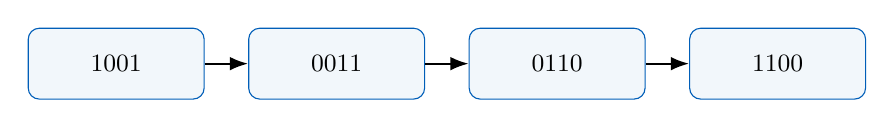
\begin{tikzpicture}[>=Latex,b/.style={draw=UOSBlue,fill=UOSBlue!5,rounded corners,minimum height=0.9cm,text width=2cm,align=center},font=\small]\node[b] (n0) at (0,0) {1001};
\node[b] (n1) at (2.8,0) {0011};\draw[->,thick] (n0) -- (n1);
\node[b] (n2) at (5.6,0) {0110};\draw[->,thick] (n1) -- (n2);
\node[b] (n3) at (8.399999999999999,0) {1100};\draw[->,thick] (n2) -- (n3);\end{tikzpicture}\end{center}\begin{itemize}\setlength{\itemsep}{0.5em}\item 네 위상을 순환시키는 2상 여자 패턴이다. 두 출력이 동시에 1이다.
\item 새 stepper\_sequence는 enable마다 비트를 회전시킨다.
\item 회전 방향은 위상 순서에 달려 있다. 실제 전류 구동과 기계 동작은 범위 밖이다.\end{itemize}
\sourceref{5.1\_클럭의 이해와 순서 논리 회로, p.73}
\end{frame}
\begin{frame}[t]{실습 18 / 핀 참고}
\fontsize{8}{9}\selectfont
원래 예제의 포트 이름과 패키지 핀. 새 시뮬레이션 탑에는 적용하지 않는다.
\begin{center}\renewcommand{\arraystretch}{1.0}
\begin{tabular}{ll@{\hspace{1.1cm}}ll}\toprule
포트 & 핀 & 포트 & 핀\\\midrule
\texttt{rst} & K4 & \texttt{stepmotor[2]} & Y22 \\
\texttt{stepmotor[3]} & Y20 & \texttt{stepmotor[1]} & AA20 \\
\texttt{clk} & B6 & \texttt{stepmotor[0]} & AA21 \\\bottomrule\end{tabular}\end{center}
{\scriptsize \par}
\sourceref{5.1\_클럭의 이해와 순서 논리 회로, p.85}\end{frame}

\checkpage{실습 18 / 스텝 모터 제어}{tb_legacy.dut.u_waveform.u_motor}{enable=1인 상승 에지마다 phase를 확인한다.}{1001→0011→0110→1100→1001 순환이며 enable=0이면 유지된다.}
\codepage{실습 18 / 스텝 모터 제어}{codesnap/src__waveform__stepper_sequence__01.png}{336}{166}{src/waveform/stepper_sequence.v}{1-12}{code:src/waveform/stepper_sequence.v}
\codepage{실습 18 / 스텝 모터 제어}{codesnap/src__waveform__stepper_sequence__01.png}{76}{790}{src/waveform/stepper_sequence.v}{13-17}{}
\subsection{실습 26 / 데이터의 저장과 이동}
\begin{frame}[t]{실습 26 / 데이터의 저장과 이동}
\small
\begin{center}\begin{tikzpicture}[>=Latex,b/.style={draw=UOSBlue,fill=UOSBlue!5,rounded corners,minimum height=0.9cm,text width=2cm,align=center},font=\small]\node[b] (n0) at (0,0) {입력 데이터};
\node[b] (n1) at (2.8,0) {저장 레지스터};\draw[->,thick] (n0) -- (n1);
\node[b] (n2) at (5.6,0) {출력 데이터};\draw[->,thick] (n1) -- (n2);\end{tikzpicture}\end{center}\begin{itemize}\setlength{\itemsep}{0.5em}\item 원자료는 저장 버튼과 Load 버튼을 분리한 4비트 저장 예시다.
\item 레지스터는 에지에서 입력을 기억하고 그 뒤 입력이 달라져도 유지한다.
\item \texttt{register4}의 save는 저장, show는 출력 갱신이다. 동시에 1이면 이전 저장값이 출력된다.\end{itemize}
\sourceref{6.2\_데이터의 저장, p.4}
\end{frame}
\begin{frame}[t]{실습 26 / 핀 참고}
\fontsize{8}{9}\selectfont
원래 예제의 포트 이름과 패키지 핀. 새 시뮬레이션 탑에는 적용하지 않는다.
\begin{center}\renewcommand{\arraystretch}{1.0}
\begin{tabular}{ll@{\hspace{1.1cm}}ll}\toprule
포트 & 핀 & 포트 & 핀\\\midrule
\texttt{sw\_s} & K4 & \texttt{o[2]} & M4 \\
\texttt{sw\_l} & N8 & \texttt{i[1]} & U2 \\
\texttt{i[3]} & Y1 & \texttt{o[1]} & M2 \\
\texttt{o[3]} & L4 & \texttt{i[0]} & T1 \\
\texttt{i[2]} & W3 & \texttt{o[0]} & N7 \\\bottomrule\end{tabular}\end{center}
{\scriptsize \par}
\sourceref{6.2\_데이터의 저장, p.16}\end{frame}

\checkpage{실습 26 / 데이터의 저장과 이동}{tb_legacy.dut.u_seq.u_register4}{save로 data를 저장한 뒤 data를 바꾸고 show를 준다.}{출력은 저장값이다. save와 show가 동시에 1이면 출력에는 이전 stored가 반영된다.}
\codepage{실습 26 / 데이터의 저장과 이동}{codesnap/src__sequential__register4__01.png}{804}{166}{src/sequential/register4.v}{1-12}{code:src/sequential/register4.v}
\codepage{실습 26 / 데이터의 저장과 이동}{codesnap/src__sequential__register4__01.png}{180}{790}{src/sequential/register4.v}{13-24}{}
\codepage{실습 26 / 데이터의 저장과 이동}{codesnap/src__sequential__register4__01.png}{76}{1414}{src/sequential/register4.v}{25-26}{}
\subsection{실습 27 / 시프트 레지스터 구현}
\begin{frame}[t]{실습 27 / 시프트 레지스터 구현}
\small
\begin{center}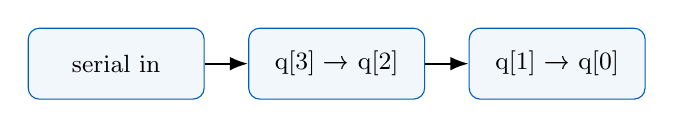
\begin{tikzpicture}[>=Latex,b/.style={draw=UOSBlue,fill=UOSBlue!5,rounded corners,minimum height=0.9cm,text width=2cm,align=center},font=\small]\node[b] (n0) at (0,0) {serial in};
\node[b] (n1) at (2.8,0) {q[3] → q[2]};\draw[->,thick] (n0) -- (n1);
\node[b] (n2) at (5.6,0) {q[1] → q[0]};\draw[->,thick] (n1) -- (n2);\end{tikzpicture}\end{center}\begin{itemize}\setlength{\itemsep}{0.5em}\item 원자료는 q[3]에서 q[0] 방향으로 이동한다.
\item \texttt{shift\_register4}는 \texttt{\{serial\_in, value[3:1]\}}로 MSB에 새 비트를 넣는다.
\item 0에서 입력 1, 0을 차례로 수락하면 1000, 0100이다. 8비트 보충 예제와 방향을 구분한다.\end{itemize}
\sourceref{6.2\_데이터의 저장, p.31, 32}
\end{frame}

\begin{frame}[t]{실습 27 / 핀 참고}
\fontsize{8}{9}\selectfont
원래 예제의 포트 이름과 패키지 핀. 새 시뮬레이션 탑에는 적용하지 않는다.
\begin{center}\renewcommand{\arraystretch}{1.0}
\begin{tabular}{ll@{\hspace{1.1cm}}ll}\toprule
포트 & 핀 & 포트 & 핀\\\midrule
\texttt{i} & K4 & \texttt{o[2]} & M4 \\
\texttt{o[3]} & L4 & \texttt{o[1]} & M2 \\
\texttt{clk} & N8 & \texttt{o[0]} & N7 \\\bottomrule\end{tabular}\end{center}
{\scriptsize \par}
\sourceref{6.2\_데이터의 저장, p.44}\end{frame}

\checkpage{실습 27 / 시프트 레지스터}{tb_legacy.dut.u_seq.u_shift4}{초기값 0000에서 serial\_in=1,0을 차례로 수락시킨다.}{value는 1000,0100이다. enable=0일 때에는 이동하지 않는다.}
\codepage{실습 27 / 시프트 레지스터}{codesnap/src__sequential__shift_register4__01.png}{388}{166}{src/sequential/shift_register4.v}{1-12}{code:src/sequential/shift_register4.v}
\codepage{실습 27 / 시프트 레지스터}{codesnap/src__sequential__shift_register4__01.png}{76}{790}{src/sequential/shift_register4.v}{13-18}{}
\subsection{실습 28 / PISO 제어}
\begin{frame}[t]{실습 28 / PISO 제어}
\small
\begin{columns}[T,onlytextwidth]\begin{column}{0.47\textwidth}\begin{center}\renewcommand{\arraystretch}{1.12}\begin{tabular}{ccc}\hline 동작 & 레지스터 & 직렬 출력\\\hline 병렬 적재 & 1010 & 1\\
1회 이동 & 0100 & 0\\
2회 이동 & 1000 & 1\\
3회 이동 & 0000 & 0\\\hline\end{tabular}\end{center}\end{column}\begin{column}{0.49\textwidth}\begin{itemize}\setlength{\itemsep}{0.5em}\item PISO는 병렬 입력·직렬 출력이다. 표는 MSB-first 예시다.
\item 출력 비트를 읽은 뒤 시프트해야 첫 비트를 놓치지 않는다.
\item 원자료 shldn=1은 적재, 0은 출력이다. 새 코드는 load와 enable을 분리한다.\end{itemize}\end{column}\end{columns}
\sourceref{6.2\_데이터의 저장, p.64}
\end{frame}
\begin{frame}[t]{실습 28 / 핀 참고}
\fontsize{8}{9}\selectfont
원래 예제의 포트 이름과 패키지 핀. 새 시뮬레이션 탑에는 적용하지 않는다.
\begin{center}\renewcommand{\arraystretch}{1.0}
\begin{tabular}{ll@{\hspace{1.1cm}}ll}\toprule
포트 & 핀 & 포트 & 핀\\\midrule
\texttt{clk} & K4 & \texttt{d[3]} & Y1 \\
\texttt{d[1]} & U2 & \texttt{d[2]} & W3 \\
\texttt{shldn} & N8 & \texttt{q} & L4 \\
\texttt{d[0]} & T1 & \texttt{} &  \\\bottomrule\end{tabular}\end{center}
{\scriptsize \par}
\sourceref{6.2\_데이터의 저장, p.76}\end{frame}

\checkpage{실습 28 / PISO 제어}{tb_legacy.dut.u_seq.u_piso4}{load=1로 1010을 적재한 뒤 load=0, enable=1로 이동한다.}{serial\_out을 이동 전에 읽으면 1,0,1,0이다. load가 enable보다 우선한다.}
\codepage{실습 28 / PISO 제어}{codesnap/src__sequential__piso4__01.png}{596}{166}{src/sequential/piso4.v}{1-12}{code:src/sequential/piso4.v}
\codepage{실습 28 / PISO 제어}{codesnap/src__sequential__piso4__01.png}{76}{790}{src/sequential/piso4.v}{13-22}{}
\section{표시 장치}
\chaptercontents{3}{표시 장치 / 구성}
\subsection{실습 10 / BCD-2진 코드 변환기}
\begin{frame}[t]{실습 10 / BCD-2진 코드 변환기}
\small
\begin{columns}[T,onlytextwidth]\begin{column}{0.47\textwidth}\begin{center}\renewcommand{\arraystretch}{1.12}\begin{tabular}{ccc}\hline 십의 자리 & 일의 자리 & 2진수 결과\\\hline 0 & 0 & 0000000\\
0 & 9 & 0001001\\
1 & 0 & 0001010\\
4 & 2 & 0101010\\
9 & 9 & 1100011\\\hline\end{tabular}\end{center}\end{column}\begin{column}{0.49\textwidth}\begin{itemize}\setlength{\itemsep}{0.5em}\item 기존 제목의 ‘2비트’는 ‘2진 코드’로 바로잡는다. 결과는 7비트다.
\item $bin=10\times ten+one$. 각 BCD 자리는 0~9만 유효하다.
\item \texttt{bcd\_to\_binary}는 BCD를 이진수로 바꾼다. 자리값이 10 이상이면 valid=0, binary=0이다.\end{itemize}\end{column}\end{columns}
\sourceref{4.1\_고급 조합논리 회로 설계, p.41, 42}
\end{frame}

\begin{frame}[t]{실습 10 / 핀 참고}
\fontsize{8}{9}\selectfont
원래 예제의 포트 이름과 패키지 핀. 새 시뮬레이션 탑에는 적용하지 않는다.
\begin{center}\renewcommand{\arraystretch}{1.0}
\begin{tabular}{ll@{\hspace{1.1cm}}ll}\toprule
포트 & 핀 & 포트 & 핀\\\midrule
\texttt{ten[3]} & Y1 & \texttt{one[3]} & W4 \\
\texttt{bin[6]} & L4 & \texttt{bin[2]} & M7 \\
\texttt{ten[2]} & W3 & \texttt{one[2]} & W1 \\
\texttt{bin[5]} & M4 & \texttt{bin[1]} & M3 \\
\texttt{ten[1]} & U2 & \texttt{one[1]} & V4 \\
\texttt{bin[4]} & M2 & \texttt{bin[0]} & M1 \\
\texttt{ten[0]} & T1 & \texttt{one[0]} & U4 \\
\texttt{bin[3]} & N7 & \texttt{} &  \\\bottomrule\end{tabular}\end{center}
{\scriptsize \par}
\sourceref{4.1\_고급 조합논리 회로 설계, p.56}\end{frame}

\checkpage{실습 10 / BCD-2진 코드 변환기}{tb_legacy.dut.u_display.u_bcd}{tens=4, ones=2이면 binary=42, valid=1이다.}{tens 또는 ones가 10 이상이면 valid=0, binary=0이다.}
\codepage{실습 10 / BCD-2진 코드 변환기}{codesnap/src__display__bcd_to_binary__01.png}{232}{166}{src/display/bcd_to_binary.v}{1-12}{code:src/display/bcd_to_binary.v}
\codepage{실습 10 / BCD-2진 코드 변환기}{codesnap/src__display__bcd_to_binary__01.png}{76}{790}{src/display/bcd_to_binary.v}{13-15}{}
\subsection{실습 11 / 7-SEGMENT DECODER 설계}
\begin{frame}[t]{실습 11 / 7-SEGMENT DECODER 설계}
\small
\begin{columns}[T,onlytextwidth]\begin{column}{0.47\textwidth}\begin{center}\renewcommand{\arraystretch}{1.12}\begin{tabular}{cc}\hline 숫자 & abcdefg\\\hline 0 & 1111110\\
1 & 0110000\\
2 & 1101101\\
3 & 1111001\\
4 & 0110011\\
5 & 1011011\\
6 & 1011111\\
7 & 1110000\\
8 & 1111111\\
9 & 1111011\\\hline\end{tabular}\end{center}\end{column}\begin{column}{0.49\textwidth}\begin{itemize}\setlength{\itemsep}{0.5em}\item 1은 점등이다. a~g 순서와 소수점 dp를 먼저 정의한다.
\item 원자료의 5·6·7 BCD 입력 오타를 0101·0110·0111로 바로잡았다.
\item 새 hex7seg는 0~F를 표시하며 \texttt{\{a,b,c,d,e,f,g,dp\}} 순서다.\end{itemize}\end{column}\end{columns}
\sourceref{4.1\_고급 조합논리 회로 설계, p.78, 79, 80}
\end{frame}


\begin{frame}[t]{실습 11 / 핀 참고}
\fontsize{8}{9}\selectfont
원래 예제의 포트 이름과 패키지 핀. 새 시뮬레이션 탑에는 적용하지 않는다.
\begin{center}\renewcommand{\arraystretch}{1.0}
\begin{tabular}{ll@{\hspace{1.1cm}}ll}\toprule
포트 & 핀 & 포트 & 핀\\\midrule
\texttt{bcd[3]} & Y1 & \texttt{bcd[0]} & Y5 \\
\texttt{seg\_data[5]} & N4 & \texttt{seg\_data[2]} & M5 \\
\texttt{bcd[2]} & W3 & \texttt{seg\_data[7]} & P1 \\
\texttt{seg\_data[4]} & N3 & \texttt{seg\_data[2]} & M4 \\
\texttt{bcd[1]} & Y4 & \texttt{seg\_data[6]} & N5 \\
\texttt{seg\_data[3]} & N1 & \texttt{seg\_data[0]} & M3 \\\bottomrule\end{tabular}\end{center}
{\scriptsize 원표에 중복 포트/핀 표기가 있다. 그대로 기록했으며 실제 배선값으로 확정하지 않는다.\par seg\_data[2]가 두 번 나타나는 원표의 인덱스 오류를 임의 수정하지 않았다.\par}
\sourceref{4.1\_고급 조합논리 회로 설계, p.94}\end{frame}

\checkpage{실습 11 / 7-SEGMENT DECODER}{tb_legacy.dut.u_display.u_manual.u_decoder}{value=0,1,8,F를 차례로 넣는다.}{segments는 abcdefg,dp 순서다. 8의 출력은 11111110이며 dp는 0이다.}
\codepage{실습 11 / 7-SEGMENT DECODER}{codesnap/src__display__hex7seg__01.png}{1116}{166}{src/display/hex7seg.v}{1-12}{code:src/display/hex7seg.v}
\codepage{실습 11 / 7-SEGMENT DECODER}{codesnap/src__display__hex7seg__01.png}{492}{790}{src/display/hex7seg.v}{13-24}{}
\codepage{실습 11 / 7-SEGMENT DECODER}{codesnap/src__display__hex7seg__01.png}{76}{1414}{src/display/hex7seg.v}{25-32}{}
\subsection{실습 12 / 7-SEGMENT ARRAY 제어}
\begin{frame}[t]{실습 12 / 7-SEGMENT ARRAY 제어}
\small
\begin{center}\begin{tikzpicture}[>=Latex,b/.style={draw=UOSBlue,fill=UOSBlue!5,rounded corners,minimum height=0.9cm,text width=2cm,align=center},font=\small]\node[b] (n0) at (0,0) {표시할 숫자};
\node[b] (n1) at (2.8,0) {7세그먼트 변환};\draw[->,thick] (n0) -- (n1);
\node[b] (n2) at (5.6,0) {자리 선택};\draw[->,thick] (n1) -- (n2);\end{tikzpicture}\end{center}\begin{itemize}\setlength{\itemsep}{0.5em}\item segment 데이터와 자리 선택 신호는 다른 역할이다.
\item \texttt{segment\_select8}은 position=0~7로 한 자리를 선택한다. 버튼 입력 처리는 포함하지 않는다.
\item 선택한 자리의 숫자와 segment 데이터가 맞는지 확인한다.\end{itemize}
\sourceref{4.1\_고급 조합논리 회로 설계, p.116, 117}
\end{frame}

\begin{frame}[t]{실습 12 / 핀 참고}
\fontsize{8}{9}\selectfont
원래 예제의 포트 이름과 패키지 핀. 새 시뮬레이션 탑에는 적용하지 않는다.
\begin{center}\renewcommand{\arraystretch}{1.0}
\begin{tabular}{ll@{\hspace{1.1cm}}ll}\toprule
포트 & 핀 & 포트 & 핀\\\midrule
\texttt{bcd[3]} & Y1 & \texttt{sw[0]} & N4 \\
\texttt{seg\_com[3]} & L6 & \texttt{seg\_data[5]} & E2 \\
\texttt{bcd[2]} & W3 & \texttt{seg\_data[4]} & E4 \\
\texttt{seg\_com[2]} & K1 & \texttt{seg\_com[7]} & H4 \\
\texttt{bcd[1]} & Y4 & \texttt{seg\_data[3]} & J1 \\
\texttt{seg\_com[1]} & K3 & \texttt{seg\_com[6]} & H6 \\
\texttt{bcd[0]} & Y5 & \texttt{seg\_data[2]} & J3 \\
\texttt{seg\_com[0]} & K5 & \texttt{seg\_com[5]} & G1 \\
\texttt{sw[2]} & K4 & \texttt{seg\_data[1]} & J7 \\
\texttt{seg\_data[7]} & F1 & \texttt{seg\_com[4]} & G3 \\
\texttt{sw[1]} & N8 & \texttt{seg\_data[0]} & H2 \\
\texttt{seg\_data[6]} & F5 & \texttt{} &  \\\bottomrule\end{tabular}\end{center}
{\scriptsize \par}
\sourceref{4.1\_고급 조합논리 회로 설계, p.131}\end{frame}

\checkpage{실습 12 / 7-SEGMENT ARRAY 제어}{tb_legacy.dut.u_display.u_manual}{digit를 고정하고 position을 0부터 7까지 바꾼다.}{digit\_select만 이동하고 segments는 유지된다. 두 신호의 역할을 분리해서 본다.}
\codepage{실습 12 / 7-SEGMENT ARRAY 제어}{codesnap/src__display__segment_select8__01.png}{388}{166}{src/display/segment_select8.v}{1-12}{code:src/display/segment_select8.v}
\codepage{실습 12 / 7-SEGMENT ARRAY 제어}{codesnap/src__display__segment_select8__01.png}{76}{790}{src/display/segment_select8.v}{13-18}{}
\subsection{실습 32 / TEXT LCD 제어}
\begin{frame}[t]{실습 32 / TEXT LCD 제어}
\small
\begin{columns}[T,onlytextwidth]\begin{column}{0.47\textwidth}\begin{center}\renewcommand{\arraystretch}{1.12}\begin{tabular}{cccc}\hline 단계 & RS & data & 의미\\\hline 0 & 0 & 38h & 8비트·2줄\\
1 & 0 & 0Ch & 표시 켜기\\
2 & 0 & 06h & 주소 증가\\
3 & 0 & 80h & 첫 줄 시작\\
4 & 1 & 48h & 문자 H\\\hline\end{tabular}\end{center}\end{column}\begin{column}{0.49\textwidth}\begin{itemize}\setlength{\itemsep}{0.5em}\item RS=0은 명령, RS=1은 문자 데이터다. E 펄스로 전달 시점을 알린다.
\item 전송 순서는 데이터 설정 → E=1 → E=0이다. 명령 4개 뒤 Hello World의 11문자를 보낸다.
\item 문자열 끝에서 첫 줄 주소 명령으로 돌아간다. 실제 LCD 초기화 대기 시간은 범위 밖이다.\end{itemize}\end{column}\end{columns}
\sourceref{8.1.CHARACTER LCD 제어, p.13}
\end{frame}
\begin{frame}[t]{실습 32 / 핀 참고}
\fontsize{8}{9}\selectfont
원래 예제의 포트 이름과 패키지 핀. 새 시뮬레이션 탑에는 적용하지 않는다.
\begin{center}\renewcommand{\arraystretch}{1.0}
\begin{tabular}{ll@{\hspace{1.1cm}}ll}\toprule
포트 & 핀 & 포트 & 핀\\\midrule
\texttt{rst} & K4 & \texttt{lcd\_data[6]} & C1 \\
\texttt{lcd\_data[3]} & D4 & \texttt{lcd\_e} & A6 \\
\texttt{clk} & B6 & \texttt{lcd\_data[5]} & C5 \\
\texttt{lcd\_data[2]} & C3 & \texttt{lcd\_rs} & G6 \\
\texttt{lcd\_data[1]} & B2 & \texttt{lcd\_data[4]} & A2 \\
\texttt{lcd\_data[7]} & D1 & \texttt{lcd\_rw} & D6 \\
\texttt{lcd\_data[0]} & A4 & \texttt{} &  \\\bottomrule\end{tabular}\end{center}
{\scriptsize \par}
\sourceref{8.1.CHARACTER LCD 제어, p.30}\end{frame}

\checkpage{실습 32 / TEXT LCD 제어}{tb_legacy.dut.u_display.u_lcd}{data,rs,e를 함께 본다. 명령 38h,0Ch,06h,80h 뒤 문자열이 나온다.}{E의 하강 에지에서 Hello World 11문자를 확인한다. 데이터 설정과 전송 에지를 구분한다.}
\codepage{실습 32 / TEXT LCD 제어}{codesnap/src__display__lcd_sequence__01.png}{1220}{166}{src/display/lcd_sequence.v}{1-12}{code:src/display/lcd_sequence.v}
\codepage{실습 32 / TEXT LCD 제어}{codesnap/src__display__lcd_sequence__01.png}{596}{790}{src/display/lcd_sequence.v}{13-24}{}
\codepage{실습 32 / TEXT LCD 제어}{codesnap/src__display__lcd_sequence__01.png}{76}{1414}{src/display/lcd_sequence.v}{25-34}{}
\codepage{실습 32 / TEXT LCD 제어}{codesnap/src__display__lcd_sequence__02.png}{960}{166}{src/display/lcd_sequence.v}{35-46}{}
\codepage{실습 32 / TEXT LCD 제어}{codesnap/src__display__lcd_sequence__02.png}{336}{790}{src/display/lcd_sequence.v}{47-58}{}
\codepage{실습 32 / TEXT LCD 제어}{codesnap/src__display__lcd_sequence__02.png}{76}{1414}{src/display/lcd_sequence.v}{59-63}{}
\section{파형 생성과 구동}
\chaptercontents{4}{파형 생성과 구동 / 구성}
\subsection{실습 19 / PIEZO 제어}
\begin{frame}[t]{실습 19 / PIEZO 제어}
\small
\begin{center}\begin{tikzpicture}[>=Latex,b/.style={draw=UOSBlue,fill=UOSBlue!5,rounded corners,minimum height=0.9cm,text width=2cm,align=center},font=\small]\node[b] (n0) at (0,0) {기준 클록};
\node[b] (n1) at (2.8,0) {N회 카운트};\draw[->,thick] (n0) -- (n1);
\node[b] (n2) at (5.6,0) {출력 반전};\draw[->,thick] (n1) -- (n2);\end{tikzpicture}\end{center}\begin{itemize}\setlength{\itemsep}{0.5em}\item 주기적으로 반전시키면 사각파가 된다. $f=f_{clk}/(2N)$.
\item 원자료는 1 MHz 입력을 분주한다.
\item 새 tone\_generator의 반주기는 16+2×note 클록이다. 실제 음계가 아닌 원리 관찰용이다.\end{itemize}
\sourceref{5.2\_클럭과 카운터 회로의 응용, p.4}
\end{frame}
\begin{frame}[t]{실습 19 / 핀 참고}
\fontsize{8}{9}\selectfont
원래 예제의 포트 이름과 패키지 핀. 새 시뮬레이션 탑에는 적용하지 않는다.
\begin{center}\renewcommand{\arraystretch}{1.0}
\begin{tabular}{ll@{\hspace{1.1cm}}ll}\toprule
포트 & 핀 & 포트 & 핀\\\midrule
\texttt{rst} & K4 & \texttt{clk} & B6 \\
\texttt{piezo} & Y21 & \texttt{} &  \\\bottomrule\end{tabular}\end{center}
{\scriptsize \par}
\sourceref{5.2\_클럭과 카운터 회로의 응용, p.16}\end{frame}

\checkpage{실습 19 / PIEZO 제어}{tb_legacy.dut.u_waveform.u_tone}{note를 고정하고 tone의 두 전환 사이 클록 수를 센다.}{반주기는 16+2 곱하기 note 클록이다. 이것을 두 배 하면 전체 주기다.}
\codepage{실습 19 / PIEZO 제어}{codesnap/src__waveform__tone_generator__01.png}{908}{166}{src/waveform/tone_generator.v}{1-12}{code:src/waveform/tone_generator.v}
\codepage{실습 19 / PIEZO 제어}{codesnap/src__waveform__tone_generator__01.png}{284}{790}{src/waveform/tone_generator.v}{13-24}{}
\codepage{실습 19 / PIEZO 제어}{codesnap/src__waveform__tone_generator__01.png}{76}{1414}{src/waveform/tone_generator.v}{25-28}{}
\subsection{실습 20 / PIEZO로 피아노 만들기}
\begin{frame}[t]{실습 20 / PIEZO로 피아노 만들기}
\small
\begin{center}\begin{tikzpicture}[>=Latex,b/.style={draw=UOSBlue,fill=UOSBlue!5,rounded corners,minimum height=0.9cm,text width=2cm,align=center},font=\small]\node[b] (n0) at (0,0) {키 입력};
\node[b] (n1) at (2.8,0) {분주값 선택};\draw[->,thick] (n0) -- (n1);
\node[b] (n2) at (5.6,0) {음원 발생};\draw[->,thick] (n1) -- (n2);\end{tikzpicture}\end{center}\begin{itemize}\setlength{\itemsep}{0.5em}\item 키마다 다른 분주값을 선택하면 다른 높이의 음을 만든다.
\item 여러 키의 우선순위와 아무 키도 없을 때의 무음을 정의한다.
\item \texttt{piano}는 8키 중 MSB 우선으로 선택한다. 무입력은 무음이며 반주기 4+note는 관찰용 값이다.\end{itemize}
\sourceref{5.2\_클럭과 카운터 회로의 응용, p.29}
\end{frame}
\begin{frame}[t]{실습 20 / 핀 참고}
\fontsize{8}{9}\selectfont
원래 예제의 포트 이름과 패키지 핀. 새 시뮬레이션 탑에는 적용하지 않는다.
\begin{center}\renewcommand{\arraystretch}{1.0}
\begin{tabular}{ll@{\hspace{1.1cm}}ll}\toprule
포트 & 핀 & 포트 & 핀\\\midrule
\texttt{rst} & Y1 & \texttt{key[6]} & N8 \\
\texttt{key[3]} & P6 & \texttt{key[0]} & J2 \\
\texttt{clk} & B6 & \texttt{key[5]} & N4 \\
\texttt{key[2]} & N6 & \texttt{key[4]} & N1 \\
\texttt{key[7]} & K4 & \texttt{piezo} & Y21 \\
\texttt{key[1]} & L5 & \texttt{} &  \\\bottomrule\end{tabular}\end{center}
{\scriptsize \par}
\sourceref{5.2\_클럭과 카운터 회로의 응용, p.41}\end{frame}

\checkpage{실습 20 / PIEZO로 피아노 만들기}{tb_legacy.dut.u_waveform.u_piano}{한 키씩 누른 뒤 무입력과 동시 입력을 검사한다.}{MSB 키가 우선한다. 선택 음이 바뀌거나 무음에서 시작하면 위상을 초기화한다.}
\codepage{실습 20 / PIEZO로 피아노 만들기}{codesnap/src__waveform__piano__01.png}{1220}{166}{src/waveform/piano.v}{1-12}{code:src/waveform/piano.v}
\codepage{실습 20 / PIEZO로 피아노 만들기}{codesnap/src__waveform__piano__01.png}{596}{790}{src/waveform/piano.v}{13-24}{}
\codepage{실습 20 / PIEZO로 피아노 만들기}{codesnap/src__waveform__piano__01.png}{76}{1414}{src/waveform/piano.v}{25-34}{}
\codepage{실습 20 / PIEZO로 피아노 만들기}{codesnap/src__waveform__piano__02.png}{284}{166}{src/waveform/piano.v}{35-46}{}
\codepage{실습 20 / PIEZO로 피아노 만들기}{codesnap/src__waveform__piano__02.png}{76}{790}{src/waveform/piano.v}{47-50}{}
\subsection{실습 21 / 시계 만들기}
\begin{frame}[t]{실습 21 / 시계 만들기}
\small
\begin{center}\begin{tikzpicture}[>=Latex,b/.style={draw=UOSBlue,fill=UOSBlue!5,rounded corners,minimum height=0.9cm,text width=2cm,align=center},font=\small]\node[b] (n0) at (0,0) {1초 tick};
\node[b] (n1) at (2.8,0) {초 → 분 카운터};\draw[->,thick] (n0) -- (n1);
\node[b] (n2) at (5.6,0) {자리별 표시};\draw[->,thick] (n1) -- (n2);\end{tikzpicture}\end{center}\begin{itemize}\setlength{\itemsep}{0.5em}\item 초가 59에서 넘어갈 때 분을 증가시킨다.
\item 시간 계수와 표시 스캔은 다른 주기다. 같은 기준 클록에서 enable을 나눈다.
\item \texttt{watch\_mmss}에서 00:59→01:00, 59:59→00:00을 검사한다. tick 한 번을 1초로 간주한다.\end{itemize}
\sourceref{5.2\_클럭과 카운터 회로의 응용, p.54}
\end{frame}
\begin{frame}[t]{실습 21 / 핀 참고}
\fontsize{8}{9}\selectfont
원래 예제의 포트 이름과 패키지 핀. 새 시뮬레이션 탑에는 적용하지 않는다.
\begin{center}\renewcommand{\arraystretch}{1.0}
\begin{tabular}{ll@{\hspace{1.1cm}}ll}\toprule
포트 & 핀 & 포트 & 핀\\\midrule
\texttt{rst} & K4 & \texttt{seg\_data[4]} & E4 \\
\texttt{seg\_com[1]} & K3 & \texttt{seg\_com[5]} & G1 \\
\texttt{clk} & B6 & \texttt{seg\_data[3]} & J1 \\
\texttt{seg\_com[0]} & K5 & \texttt{seg\_com[4]} & G3 \\
\texttt{seg\_data[7]} & F1 & \texttt{seg\_data[2]} & J3 \\
\texttt{seg\_data[6]} & F5 & \texttt{seg\_com[3]} & L6 \\
\texttt{seg\_com[7]} & H4 & \texttt{seg\_data[2]} & J7 \\
\texttt{seg\_data[5]} & E2 & \texttt{seg\_com[2]} & K1 \\
\texttt{seg\_com[6]} & H6 & \texttt{seg\_data[0]} & H2 \\\bottomrule\end{tabular}\end{center}
{\scriptsize 원표에 중복 포트/핀 표기가 있다. 그대로 기록했으며 실제 배선값으로 확정하지 않는다.\par seg\_data[2]가 두 번 나타나는 원표의 인덱스 오류를 임의 수정하지 않았다.\par}
\sourceref{5.2\_클럭과 카운터 회로의 응용, p.70}\end{frame}

\checkpage{실습 21 / 시계 만들기}{tb_legacy.dut.u_waveform.u_watch}{tick=1인 상승 에지를 1초로 간주하여 초와 분을 증가시킨다.}{00:59→01:00, 59:59→00:00을 확인한다. 자리 스캔은 tick과 별도로 계속 진행한다.}
\codepage{실습 21 / 시계 만들기}{codesnap/src__waveform__watch_mmss__01.png}{1220}{166}{src/waveform/watch_mmss.v}{1-12}{code:src/waveform/watch_mmss.v}
\codepage{실습 21 / 시계 만들기}{codesnap/src__waveform__watch_mmss__01.png}{596}{790}{src/waveform/watch_mmss.v}{13-24}{}
\codepage{실습 21 / 시계 만들기}{codesnap/src__waveform__watch_mmss__01.png}{76}{1414}{src/waveform/watch_mmss.v}{25-34}{}
\codepage{실습 21 / 시계 만들기}{codesnap/src__waveform__watch_mmss__02.png}{128}{166}{src/waveform/watch_mmss.v}{35-46}{}
\codepage{실습 21 / 시계 만들기}{codesnap/src__waveform__watch_mmss__02.png}{76}{790}{src/waveform/watch_mmss.v}{47-47}{}
\subsection{실습 22 / PWM을 이용한 LED 밝기 제어}
\begin{frame}[t]{실습 22 / PWM을 이용한 LED 밝기 제어}
\small
\begin{center}\begin{tikzpicture}[x=0.4cm,y=0.8cm,>=Latex]
\draw[->,gray] (0,0)--(17,0) node[right]{클록};
\draw[UOSBlue,very thick] (0,0)--(0,1)--(4,1)--(4,0)--(16,0)--(16,1);
\draw[<->] (0,-0.5)--node[below]{16클록 중 4클록 HIGH}(16,-0.5);
\end{tikzpicture}\end{center}\begin{itemize}\setlength{\itemsep}{0.5em}\item PWM은 주기를 유지하고 1인 시간의 비율을 바꾼다.
\item 새 pwm4는 phase=0~15와 duty를 비교한다. duty=4는 25\%다.
\item duty=0은 항상 0, duty=15는 15/16이다. 이 입력 폭에는 100\% 설정이 없다.\end{itemize}
\sourceref{6.1\_PWM 회로 구현, p.7}
\end{frame}
\begin{frame}[t]{실습 22 / 핀 참고}
\fontsize{8}{9}\selectfont
원래 예제의 포트 이름과 패키지 핀. 새 시뮬레이션 탑에는 적용하지 않는다.
\begin{center}\renewcommand{\arraystretch}{1.0}
\begin{tabular}{ll@{\hspace{1.1cm}}ll}\toprule
포트 & 핀 & 포트 & 핀\\\midrule
\texttt{rst} & Y1 & \texttt{led[2]} & M3 \\
\texttt{led[5]} & M2 & \texttt{led[7]} & L4 \\
\texttt{clk} & B6 & \texttt{led[1]} & M1 \\
\texttt{led[4]} & N7 & \texttt{led[6]} & M4 \\
\texttt{sw} & K4 & \texttt{led[0]} & N5 \\
\texttt{led[3]} & M7 & \texttt{} &  \\\bottomrule\end{tabular}\end{center}
{\scriptsize \par}
\sourceref{6.1\_PWM 회로 구현, p.19}\end{frame}

\checkpage{실습 22 / PWM을 이용한 LED 밝기 제어}{tb_legacy.dut.u_waveform.u_red}{duty를 0,4,8,15로 바꾸고 phase의 16클록 구간을 센다.}{HIGH 클록 수는 각각 0,4,8,15다. 15는 100\%가 아니다.}
\codepage{실습 22 / PWM을 이용한 LED 밝기 제어}{codesnap/src__waveform__pwm4__01.png}{492}{166}{src/waveform/pwm4.v}{1-12}{code:src/waveform/pwm4.v}
\codepage{실습 22 / PWM을 이용한 LED 밝기 제어}{codesnap/src__waveform__pwm4__01.png}{76}{790}{src/waveform/pwm4.v}{13-20}{}
\subsection{실습 23 / FULL COLOR LED 순차 제어}
\begin{frame}[t]{실습 23 / FULL COLOR LED 순차 제어}
\small
\begin{columns}[T,onlytextwidth]\begin{column}{0.47\textwidth}\begin{center}\renewcommand{\arraystretch}{1.12}\begin{tabular}{cccc}\hline R & G & B & 색\\\hline 1 & 0 & 0 & 빨강\\
0 & 1 & 0 & 초록\\
0 & 0 & 1 & 파랑\\
1 & 1 & 0 & 노랑\\
1 & 1 & 1 & 흰색\\\hline\end{tabular}\end{center}\end{column}\begin{column}{0.49\textwidth}\begin{itemize}\setlength{\itemsep}{0.5em}\item RGB 세 출력을 조합한다. 모두 0이면 꺼짐이다.
\item 원자료는 버튼 입력마다 색 상태를 순환한다. 입력과 상태를 구분한다.
\item 단순 ON/OFF 색 선택과 PWM 밝기 조절은 다르다.\end{itemize}\end{column}\end{columns}
\sourceref{6.1\_PWM 회로 구현, p.34}
\end{frame}
\begin{frame}[t]{실습 23 / 핀 참고}
\fontsize{8}{9}\selectfont
원래 예제의 포트 이름과 패키지 핀. 새 시뮬레이션 탑에는 적용하지 않는다.
\begin{center}\renewcommand{\arraystretch}{1.0}
\begin{tabular}{ll@{\hspace{1.1cm}}ll}\toprule
포트 & 핀 & 포트 & 핀\\\midrule
\texttt{sw} & K4 & \texttt{cled\_r[1]} & P2 \\
\texttt{cled\_g[2]} & V1 & \texttt{cled\_b[2]} & W2 \\
\texttt{cled\_g[1]} & R7 & \texttt{cled\_r[0]} & R3 \\
\texttt{cled\_r[3]} & T2 & \texttt{cled\_b[1]} & R5 \\
\texttt{cled\_g[0]} & T6 & \texttt{cled\_g[3]} & U5 \\
\texttt{cled\_r[2]} & U1 & \texttt{cled\_b[0]} & T3 \\
\texttt{cled\_b[3]} & U3 & \texttt{} &  \\\bottomrule\end{tabular}\end{center}
{\scriptsize \par}
\sourceref{6.1\_PWM 회로 구현, p.46}\end{frame}

\checkpage{실습 23 / FULL COLOR LED 순차 제어}{tb_legacy.dut.u_waveform.u_rgb}{reset 후 rgb=100이고 next\_color마다 다음 색으로 이동한다.}{100→010→001→100이다. 원표의 혼합색 조합은 보충 설명이며 이 코드는 세 색만 순환한다.}
\codepage{실습 23 / FULL COLOR LED 순차 제어}{codesnap/src__waveform__rgb_sequence__01.png}{336}{166}{src/waveform/rgb_sequence.v}{1-12}{code:src/waveform/rgb_sequence.v}
\codepage{실습 23 / FULL COLOR LED 순차 제어}{codesnap/src__waveform__rgb_sequence__01.png}{76}{790}{src/waveform/rgb_sequence.v}{13-17}{}
\subsection{실습 24 / FULL COLOR LED PWM 제어}
\begin{frame}[t]{실습 24 / FULL COLOR LED PWM 제어}
\small
\begin{center}\begin{tikzpicture}[>=Latex,b/.style={draw=UOSBlue,fill=UOSBlue!5,rounded corners,minimum height=0.9cm,text width=2cm,align=center},font=\small]\node[b] (n0) at (0,0) {공통 phase};
\node[b] (n1) at (2.8,0) {R·G·B duty 비교};\draw[->,thick] (n0) -- (n1);
\node[b] (n2) at (5.6,0) {RGB 출력};\draw[->,thick] (n1) -- (n2);\end{tikzpicture}\end{center}\begin{itemize}\setlength{\itemsep}{0.5em}\item 세 채널은 같은 주기, 서로 다른 duty를 갖는다.
\item 새 코드는 빨강 가변, 초록 4/16, 파랑 12/16로 구성했다.
\item 여기서는 디지털 비율을 검사한다. 사람이 느끼는 밝기가 duty와 완전히 비례하는 것은 아니다.\end{itemize}
\sourceref{6.1\_PWM 회로 구현, p.61}
\end{frame}
\begin{frame}[t]{실습 24 / 핀 참고}
\fontsize{8}{9}\selectfont
원래 예제의 포트 이름과 패키지 핀. 새 시뮬레이션 탑에는 적용하지 않는다.
\begin{center}\renewcommand{\arraystretch}{1.0}
\begin{tabular}{ll@{\hspace{1.1cm}}ll}\toprule
포트 & 핀 & 포트 & 핀\\\midrule
\texttt{rst} & Y1 & \texttt{cled\_g[0]} & T6 \\
\texttt{cled\_r[0]} & R3 & \texttt{cled\_b[3]} & U3 \\
\texttt{clk} & B6 & \texttt{cled\_r[3]} & T2 \\
\texttt{cled\_g[3]} & U5 & \texttt{cled\_b[2]} & W2 \\
\texttt{sw\_r} & K4 & \texttt{cled\_r[2]} & U1 \\
\texttt{cled\_g[2]} & V1 & \texttt{cled\_b[1]} & R5 \\
\texttt{sw\_g} & N8 & \texttt{cled\_r[1]} & P2 \\
\texttt{cled\_g[1]} & R7 & \texttt{cled\_b[0]} & T3 \\
\texttt{sw\_b} & N4 & \texttt{} &  \\\bottomrule\end{tabular}\end{center}
{\scriptsize \par}
\sourceref{6.1\_PWM 회로 구현, p.74}\end{frame}

\checkpage{실습 24 / FULL COLOR LED PWM 제어}{tb_legacy.dut.u_waveform}{세 채널의 phase가 일치하는 상태에서 duty를 바꾼다.}{빨강은 가변, 초록은 4/16, 파랑은 12/16의 HIGH 비율이다.}
\codepage{실습 24 / FULL COLOR LED PWM 제어}{codesnap/src__waveform__lab_waveform__01.png}{960}{166}{src/waveform/lab_waveform.v}{1-12}{code:src/waveform/lab_waveform.v}
\codepage{실습 24 / FULL COLOR LED PWM 제어}{codesnap/src__waveform__lab_waveform__01.png}{336}{790}{src/waveform/lab_waveform.v}{13-24}{}
\codepage{실습 24 / FULL COLOR LED PWM 제어}{codesnap/src__waveform__lab_waveform__01.png}{76}{1414}{src/waveform/lab_waveform.v}{25-29}{}
\codepage{실습 24 / FULL COLOR LED PWM 제어}{codesnap/src__waveform__lab_waveform__02.png}{1168}{166}{src/waveform/lab_waveform.v}{30-41}{}
\codepage{실습 24 / FULL COLOR LED PWM 제어}{codesnap/src__waveform__lab_waveform__02.png}{544}{790}{src/waveform/lab_waveform.v}{42-53}{}
\codepage{실습 24 / FULL COLOR LED PWM 제어}{codesnap/src__waveform__lab_waveform__02.png}{76}{1414}{src/waveform/lab_waveform.v}{54-62}{}
\codepage{실습 24 / FULL COLOR LED PWM 제어}{codesnap/src__waveform__lab_waveform__03.png}{1012}{166}{src/waveform/lab_waveform.v}{63-74}{}
\codepage{실습 24 / FULL COLOR LED PWM 제어}{codesnap/src__waveform__lab_waveform__03.png}{388}{790}{src/waveform/lab_waveform.v}{75-86}{}
\codepage{실습 24 / FULL COLOR LED PWM 제어}{codesnap/src__waveform__lab_waveform__03.png}{76}{1414}{src/waveform/lab_waveform.v}{87-92}{}
\section{상태 머신}
\chaptercontents{5}{상태 머신 / 구성}
\subsection{실습 29 / 무어 스테이트 머신 설계}
\begin{frame}[t]{실습 29 / 무어 스테이트 머신 설계}
\small
\begin{center}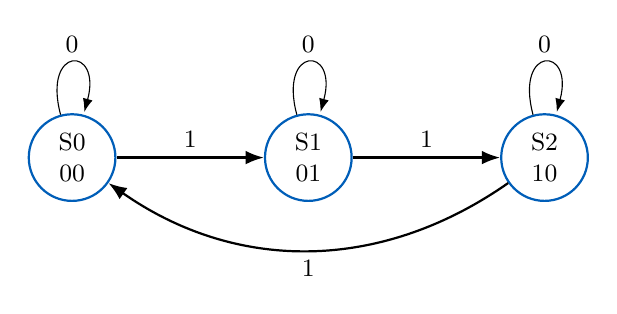
\begin{tikzpicture}[>=Latex,st/.style={circle,draw=UOSBlue,thick,minimum size=1.1cm,align=center},font=\small]
\node[st](a) at (0,0){S0\\00};\node[st](b) at (3,0){S1\\01};\node[st](c) at (6,0){S2\\10};
\path[->,thick] (a) edge node[above]{1}(b) (b) edge node[above]{1}(c) (c) edge[bend left=35] node[below]{1}(a);
\path[->] (a) edge[loop above] node{0}(a) (b) edge[loop above] node{0}(b) (c) edge[loop above] node{0}(c);
\end{tikzpicture}\end{center}\begin{itemize}\setlength{\itemsep}{0.5em}\item Moore 출력은 현재 상태로 결정된다. 원자료는 00/01/10 출력의 3상태 순환이다.
\item 입력 0은 유지, 1은 다음 상태로 진행한다.
\item \texttt{moore\_cycle}이 위 3상태를 구현한다. 보충 \texttt{moore101}은 별도의 패턴 검출기다.\end{itemize}
\sourceref{9.1\_스테이트 머신의 구현, p.4, 5}
\end{frame}

\begin{frame}[t]{실습 29 / 핀 참고}
\fontsize{8}{9}\selectfont
원래 예제의 포트 이름과 패키지 핀. 새 시뮬레이션 탑에는 적용하지 않는다.
\begin{center}\renewcommand{\arraystretch}{1.0}
\begin{tabular}{ll@{\hspace{1.1cm}}ll}\toprule
포트 & 핀 & 포트 & 핀\\\midrule
\texttt{rst} & K4 & \texttt{x} & N8 \\
\texttt{y[1]} & L4 & \texttt{y[0]} & M4 \\\bottomrule\end{tabular}\end{center}
{\scriptsize \par}
\sourceref{9.1\_스테이트 머신의 구현, p.9}\end{frame}

\checkpage{실습 29 / 무어 스테이트 머신}{tb_legacy.dut.u_fsm.u_cycle}{enable=1에서 advance를 0과 1로 바꾼다.}{0이면 상태 유지, 1이면 00→01→10→00이다. value는 현재 state와 같다.}
\codepage{실습 29 / 무어 스테이트 머신}{codesnap/src__fsm__moore_cycle__01.png}{544}{166}{src/fsm/moore_cycle.v}{1-12}{code:src/fsm/moore_cycle.v}
\codepage{실습 29 / 무어 스테이트 머신}{codesnap/src__fsm__moore_cycle__01.png}{76}{790}{src/fsm/moore_cycle.v}{13-21}{}
\subsection{실습 30 / 밀리 스테이트 머신 구현}
\begin{frame}[t]{실습 30 / 밀리 스테이트 머신 구현}
\small
\begin{center}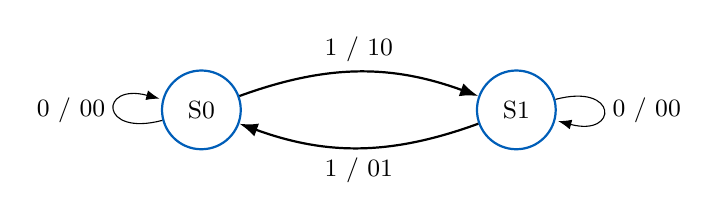
\begin{tikzpicture}[>=Latex,st/.style={circle,draw=UOSBlue,thick,minimum size=1cm},font=\small]
\node[st](a) at (0,0){S0};\node[st](b) at (4,0){S1};
\path[->,thick] (a) edge[bend left=20] node[above]{1 / 10}(b) (b) edge[bend left=20] node[below]{1 / 01}(a);
\path[->] (a) edge[loop left] node{0 / 00}(a) (b) edge[loop right] node{0 / 00}(b);
\end{tikzpicture}\end{center}\begin{itemize}\setlength{\itemsep}{0.5em}\item 화살표는 입력 / 출력이다. Mealy 출력은 상태와 현재 입력에 의해 결정된다.
\item 원자료는 입력 1마다 S0와 S1을 번갈아 이동하며 다른 값을 출력한다.
\item \texttt{mealy\_toggle}은 상태와 bit\_in으로 즉시 출력을 정한다. enable은 상태 갱신만 허용한다.\end{itemize}
\sourceref{9.1\_스테이트 머신의 구현, p.17, 18, 19}
\end{frame}


\begin{frame}[t]{실습 30 / 핀 참고}
\fontsize{8}{9}\selectfont
원래 예제의 포트 이름과 패키지 핀. 새 시뮬레이션 탑에는 적용하지 않는다.
\begin{center}\renewcommand{\arraystretch}{1.0}
\begin{tabular}{ll@{\hspace{1.1cm}}ll}\toprule
포트 & 핀 & 포트 & 핀\\\midrule
\texttt{rst} & K4 & \texttt{x} & N8 \\
\texttt{y[1]} & L4 & \texttt{y[0]} & M4 \\\bottomrule\end{tabular}\end{center}
{\scriptsize \par}
\sourceref{9.1\_스테이트 머신의 구현, p.21}\end{frame}

\checkpage{실습 30 / 밀리 스테이트 머신}{tb_legacy.dut.u_fsm.u_toggle}{bit\_in=0이면 출력 00, 1이면 상태에 따라 10 또는 01이다.}{enable=0으로 상태가 멈춰도 bit\_in이 바뀌면 출력이 달라질 수 있다.}
\codepage{실습 30 / 밀리 스테이트 머신}{codesnap/src__fsm__mealy_toggle__01.png}{492}{166}{src/fsm/mealy_toggle.v}{1-12}{code:src/fsm/mealy_toggle.v}
\codepage{실습 30 / 밀리 스테이트 머신}{codesnap/src__fsm__mealy_toggle__01.png}{76}{790}{src/fsm/mealy_toggle.v}{13-20}{}
\subsection{응용 / 상태 머신 통합 제어}
\begin{frame}[t]{응용 / 상태 머신 통합 제어}
\small
\begin{center}\begin{tikzpicture}[>=Latex,b/.style={draw=UOSBlue,fill=UOSBlue!5,rounded corners,minimum height=0.9cm,text width=2cm,align=center},font=\small]\node[b] (n0) at (0,0) {S0: 대기};
\node[b] (n1) at (2.8,0) {S1: RGB LED};\draw[->,thick] (n0) -- (n1);
\node[b] (n2) at (5.6,0) {S2: 모터};\draw[->,thick] (n1) -- (n2);\end{tikzpicture}\end{center}\begin{itemize}\setlength{\itemsep}{0.5em}\item 원자료 9.1절 p.27의 응용 과제다. 모드를 바꾸면 세 상태가 순환한다.
\item 현재 상태에 따라 RGB 또는 모터 동작을 허용하는 구조로 나눈다.
\item \texttt{mode\_controller}는 next\_mode로 모드를 바꾸고, 비활성 장치의 출력은 0으로 둔다.\end{itemize}
\sourceref{9.1\_스테이트 머신의 구현, p.27}
\end{frame}
\begin{frame}[t]{응용 / 상태 머신 통합 제어 / 핀 참고 (1)}
\fontsize{8}{9}\selectfont
원래 예제의 포트 이름과 패키지 핀. 새 시뮬레이션 탑에는 적용하지 않는다.
\begin{center}\renewcommand{\arraystretch}{1.0}
\begin{tabular}{ll@{\hspace{1.1cm}}ll}\toprule
포트 & 핀 & 포트 & 핀\\\midrule
\texttt{clk} & B6 & \texttt{seg\_com[4]} & G3 \\
\texttt{step\_motor[3]} & Y20 & \texttt{fled\_r[2]} & U1 \\
\texttt{rst} & K4 & \texttt{seg\_com[3]} & L6 \\
\texttt{step\_motor[2]} & Y22 & \texttt{fled\_r[1]} & P2 \\
\texttt{mode} & N8 & \texttt{seg\_com[2]} & K1 \\
\texttt{step\_motor[1]} & AA20 & \texttt{fled\_r[0]} & K4 \\
\texttt{step\_motor[0]} & AA21 & \texttt{seg\_com[1]} & K3 \\
\texttt{motor\_sense} & Y19 & \texttt{fled\_g[3]} & U5 \\
\texttt{seg\_com[7]} & H4 & \texttt{seg\_com[0]} & K5 \\
\texttt{seg\_com[6]} & H6 & \texttt{fled\_g[2]} & V1 \\
\texttt{seg\_com[5]} & G1 & \texttt{seg\_data[7]} & F1 \\
\texttt{fled\_r[3]} & T2 & \texttt{fled\_g[1]} & R7 \\\bottomrule\end{tabular}\end{center}
{\scriptsize 원표에 중복 포트/핀 표기가 있다. 그대로 기록했으며 실제 배선값으로 확정하지 않는다.\par fled\_r[0]=K4는 rst와 충돌한다. 다른 RGB 예제의 R3와도 다르므로 원본 XDC 대조가 필요하다.\par seg\_data[2]가 두 번 나타나는 원표의 인덱스 오류를 임의 수정하지 않았다.\par}
\sourceref{9.1\_스테이트 머신의 구현, p.28}\end{frame}
\begin{frame}[t]{응용 / 상태 머신 통합 제어 / 핀 참고 (2)}
\fontsize{8}{9}\selectfont
원래 예제의 포트 이름과 패키지 핀. 새 시뮬레이션 탑에는 적용하지 않는다.
\begin{center}\renewcommand{\arraystretch}{1.0}
\begin{tabular}{ll@{\hspace{1.1cm}}ll}\toprule
포트 & 핀 & 포트 & 핀\\\midrule
\texttt{seg\_data[6]} & F5 & \texttt{seg\_data[3]} & J1 \\
\texttt{fled\_g[0]} & T6 & \texttt{fled\_b[1]} & R5 \\
\texttt{seg\_data[5]} & E2 & \texttt{seg\_data[2]} & J3 \\
\texttt{fled\_b[3]} & U3 & \texttt{fled\_b[0]} & T3 \\
\texttt{seg\_data[4]} & E4 & \texttt{seg\_data[2]} & J7 \\
\texttt{fled\_b[2]} & W2 & \texttt{seg\_data[0]} & H2 \\\bottomrule\end{tabular}\end{center}
{\scriptsize 원표에 중복 포트/핀 표기가 있다. 그대로 기록했으며 실제 배선값으로 확정하지 않는다.\par fled\_r[0]=K4는 rst와 충돌한다. 다른 RGB 예제의 R3와도 다르므로 원본 XDC 대조가 필요하다.\par seg\_data[2]가 두 번 나타나는 원표의 인덱스 오류를 임의 수정하지 않았다.\par}
\sourceref{9.1\_스테이트 머신의 구현, p.28}\end{frame}

\checkpage{응용 / 상태 머신 통합 제어}{tb_legacy.dut.u_fsm.u_mode}{next\_mode로 대기→RGB→모터→대기를 순환한다.}{RGB 모드에서는 motor=0, 모터 모드에서는 rgb=0이다. 장치 진행은 enable로 제어한다.}
\codepage{응용 / 상태 머신 통합 제어}{codesnap/src__fsm__mode_controller__01.png}{1220}{166}{src/fsm/mode_controller.v}{1-12}{code:src/fsm/mode_controller.v}
\codepage{응용 / 상태 머신 통합 제어}{codesnap/src__fsm__mode_controller__01.png}{596}{790}{src/fsm/mode_controller.v}{13-24}{}
\codepage{응용 / 상태 머신 통합 제어}{codesnap/src__fsm__mode_controller__01.png}{76}{1414}{src/fsm/mode_controller.v}{25-34}{}
\codepage{응용 / 상태 머신 통합 제어}{codesnap/src__fsm__mode_controller__02.png}{76}{166}{src/fsm/mode_controller.v}{35-36}{}
\section{인터페이스와 통합 검증}
\chaptercontents{6}{인터페이스와 통합 검증 / 구성}
\subsection{UART 8N1}
\begin{frame}{UART 8N1}
\begin{itemize}
\item 유휴 상태는 1, 시작 비트는 0이다.
\item 8비트를 최하위 비트부터 보내고 정지 비트 1로 프레임을 마친다.
\item 송신 출력과 수신 입력을 연결한 루프백으로 256가지 바이트를 검사한다.
\item 외부 보드 입력에는 동기화가 필요하다. 현재 예제는 동일 클록 도메인의 내부 루프백이다.
\end{itemize}
\end{frame}

\checkpage{UART 8N1}{tb_legacy.dut.u_interface}{start 펄스와 data를 넣고 tx,busy,received,valid를 관찰한다.}{8N1, LSB-first다. valid가 1인 수신 완료 시점에서 received와 송신값을 비교한다.}
\codepage{UART 8N1}{codesnap/src__interface__lab_interface__01.png}{1220}{166}{src/interface/lab_interface.v}{1-12}{code:src/interface/lab_interface.v}
\codepage{UART 8N1}{codesnap/src__interface__lab_interface__01.png}{596}{790}{src/interface/lab_interface.v}{13-24}{}
\codepage{UART 8N1}{codesnap/src__interface__lab_interface__01.png}{76}{1414}{src/interface/lab_interface.v}{25-34}{}
\subsection{통합 시뮬레이션}
\begin{frame}{전체 시뮬레이션 실행}
\begin{itemize}
\item \texttt{legacy\_all\_hdl.code-workspace}를 VS Code에서 연다.
\item 빌드 태스크 \texttt{Legacy: simulate all}을 실행한다.
\item \texttt{xvlog}, \texttt{xelab}, \texttt{xsim}을 순서대로 실행한다.
\item 37개 설계 모듈, 테스트벤치 하나, 6개 계층. XSim 자동검사 20,727개 통과.
\item \texttt{build/legacy.vcd}를 VaporView에서 열고 계층별 신호를 선택한다.
\end{itemize}
\end{frame}
\begin{frame}{보드 검증과 시뮬레이션의 구분}
\begin{itemize}
\item 새 코드의 reset은 동기식 active-high다. 원자료의 reset 방식과 구분한다.
\item PWM·음원·LCD는 빠른 시뮬레이션을 위한 기능 확인용 설정이다.
\item LCD 전원 투입 초기화 시간, 모터 속도, UART baud rate는 실물 적용 전에 설정해야 한다.
\item ADC·DAC·SRAM·서보의 장비 제공 소스는 보존했다. 새 계층의 장치 모델과 검증은 후속 작업이다.
\end{itemize}
\end{frame}

\subsection{실습별 VCD 시간 구간}
\begin{frame}[t]{실습별 VCD 시간 구간 / 1}
\fontsize{8}{9}\selectfont
기준: 제공 테스트벤치 실행, 단위 ns. VCD 뷰어가 ps이면 1,000배한다.
\begin{center}\renewcommand{\arraystretch}{1.05}
\begin{tabular}{lrr}\toprule
구간 이름 & 시작(ns) & 끝(ns)\\\midrule
\texttt{01-logic-gates} & 1300 & 1340 \\
\texttt{02-not} & 1340 & 1360 \\
\texttt{03-full-adder} & 1360 & 1440 \\
\texttt{04-full-subtractor} & 1440 & 1520 \\
\texttt{05-encoder} & 1520 & 4080 \\
\texttt{06-decoder} & 4080 & 4160 \\
\texttt{07-mux} & 4160 & 4800 \\
\texttt{08-demux} & 4800 & 4960 \\
\texttt{09-compare} & 4960 & 7520 \\
\texttt{13-adder4} & 7520 & 10080 \\
\texttt{14-subtractor4} & 10080 & 12640 \\
\bottomrule\end{tabular}\end{center}
\end{frame}
\begin{frame}[t]{실습별 VCD 시간 구간 / 2}
\fontsize{8}{9}\selectfont
기준: 제공 테스트벤치 실행, 단위 ns. VCD 뷰어가 ps이면 1,000배한다.
\begin{center}\renewcommand{\arraystretch}{1.05}
\begin{tabular}{lrr}\toprule
구간 이름 & 시작(ns) & 끝(ns)\\\midrule
\texttt{15-multiplier4} & 12640 & 15200 \\
\texttt{00-first-counter} & 15200 & 15380 \\
\texttt{16-up-down-counter} & 15380 & 15540 \\
\texttt{17-divider} & 15540 & 16070 \\
\texttt{26-register} & 16070 & 16140 \\
\texttt{27-shift-register} & 16140 & 16290 \\
\texttt{28-piso} & 16290 & 16370 \\
\texttt{10-bcd-converter} & 16370 & 18960 \\
\texttt{11-seven-segment} & 18960 & 19120 \\
\texttt{12-digit-selection} & 19120 & 19200 \\
\texttt{32-lcd} & 19200 & 19680 \\
\bottomrule\end{tabular}\end{center}
\end{frame}
\begin{frame}[t]{실습별 VCD 시간 구간 / 3}
\fontsize{8}{9}\selectfont
기준: 제공 테스트벤치 실행, 단위 ns. VCD 뷰어가 ps이면 1,000배한다.
\begin{center}\renewcommand{\arraystretch}{1.05}
\begin{tabular}{lrr}\toprule
구간 이름 & 시작(ns) & 끝(ns)\\\midrule
\texttt{18-stepper} & 19680 & 19790 \\
\texttt{19-tone} & 19790 & 20460 \\
\texttt{20-piano} & 20460 & 21461 \\
\texttt{21-watch} & 21461 & 57490 \\
\texttt{22-pwm} & 57490 & 60530 \\
\texttt{23-rgb} & 60530 & 60620 \\
\texttt{24-rgb-pwm} & 60620 & 60970 \\
\texttt{29-moore} & 60970 & 61070 \\
\texttt{30-mealy} & 61070 & 61111 \\
\texttt{31-state-application} & 61111 & 61190 \\
\texttt{33-uart} & 61190 & 291620 \\
\bottomrule\end{tabular}\end{center}
\end{frame}
\subsection{통합 계층과 보충 모듈 코드}
\codepage{half\_adder.v}{codesnap/src__combinational__half_adder__01.png}{232}{166}{src/combinational/half_adder.v}{1-12}{code:src/combinational/half_adder.v}
\codepage{half\_adder.v}{codesnap/src__combinational__half_adder__01.png}{76}{790}{src/combinational/half_adder.v}{13-15}{}
\codepage{lab\_display.v}{codesnap/src__display__lab_display__01.png}{960}{166}{src/display/lab_display.v}{1-12}{code:src/display/lab_display.v}
\codepage{lab\_display.v}{codesnap/src__display__lab_display__01.png}{336}{790}{src/display/lab_display.v}{13-24}{}
\codepage{lab\_display.v}{codesnap/src__display__lab_display__01.png}{76}{1414}{src/display/lab_display.v}{25-29}{}
\codepage{lab\_display.v}{codesnap/src__display__lab_display__02.png}{1220}{166}{src/display/lab_display.v}{30-41}{}
\codepage{lab\_display.v}{codesnap/src__display__lab_display__02.png}{596}{790}{src/display/lab_display.v}{42-53}{}
\codepage{lab\_display.v}{codesnap/src__display__lab_display__02.png}{76}{1414}{src/display/lab_display.v}{54-63}{}
\codepage{lab\_display.v}{codesnap/src__display__lab_display__03.png}{76}{166}{src/display/lab_display.v}{64-73}{}
\codepage{moore101.v}{codesnap/src__fsm__moore101__01.png}{1012}{166}{src/fsm/moore101.v}{1-12}{code:src/fsm/moore101.v}
\codepage{moore101.v}{codesnap/src__fsm__moore101__01.png}{388}{790}{src/fsm/moore101.v}{13-24}{}
\codepage{moore101.v}{codesnap/src__fsm__moore101__01.png}{76}{1414}{src/fsm/moore101.v}{25-30}{}
\codepage{mealy101.v}{codesnap/src__fsm__mealy101__01.png}{908}{166}{src/fsm/mealy101.v}{1-12}{code:src/fsm/mealy101.v}
\codepage{mealy101.v}{codesnap/src__fsm__mealy101__01.png}{284}{790}{src/fsm/mealy101.v}{13-24}{}
\codepage{mealy101.v}{codesnap/src__fsm__mealy101__01.png}{76}{1414}{src/fsm/mealy101.v}{25-28}{}
\codepage{lab\_fsm.v}{codesnap/src__fsm__lab_fsm__01.png}{1220}{166}{src/fsm/lab_fsm.v}{1-12}{code:src/fsm/lab_fsm.v}
\codepage{lab\_fsm.v}{codesnap/src__fsm__lab_fsm__01.png}{596}{790}{src/fsm/lab_fsm.v}{13-24}{}
\codepage{lab\_fsm.v}{codesnap/src__fsm__lab_fsm__01.png}{76}{1414}{src/fsm/lab_fsm.v}{25-34}{}
\codepage{lab\_fsm.v}{codesnap/src__fsm__lab_fsm__02.png}{1220}{166}{src/fsm/lab_fsm.v}{35-46}{}
\codepage{lab\_fsm.v}{codesnap/src__fsm__lab_fsm__02.png}{596}{790}{src/fsm/lab_fsm.v}{47-58}{}
\codepage{lab\_fsm.v}{codesnap/src__fsm__lab_fsm__02.png}{76}{1414}{src/fsm/lab_fsm.v}{59-68}{}
\codepage{lab\_fsm.v}{codesnap/src__fsm__lab_fsm__03.png}{76}{166}{src/fsm/lab_fsm.v}{69-71}{}
\codepage{uart\_transmitter.v}{codesnap/src__interface__uart_transmitter__01.png}{1220}{166}{src/interface/uart_transmitter.v}{1-12}{code:src/interface/uart_transmitter.v}
\codepage{uart\_transmitter.v}{codesnap/src__interface__uart_transmitter__01.png}{596}{790}{src/interface/uart_transmitter.v}{13-24}{}
\codepage{uart\_transmitter.v}{codesnap/src__interface__uart_transmitter__01.png}{76}{1414}{src/interface/uart_transmitter.v}{25-34}{}
\codepage{uart\_transmitter.v}{codesnap/src__interface__uart_transmitter__02.png}{76}{166}{src/interface/uart_transmitter.v}{35-38}{}
\codepage{uart\_receiver.v}{codesnap/src__interface__uart_receiver__01.png}{1220}{166}{src/interface/uart_receiver.v}{1-12}{code:src/interface/uart_receiver.v}
\codepage{uart\_receiver.v}{codesnap/src__interface__uart_receiver__01.png}{596}{790}{src/interface/uart_receiver.v}{13-24}{}
\codepage{uart\_receiver.v}{codesnap/src__interface__uart_receiver__01.png}{76}{1414}{src/interface/uart_receiver.v}{25-34}{}
\codepage{uart\_receiver.v}{codesnap/src__interface__uart_receiver__02.png}{960}{166}{src/interface/uart_receiver.v}{35-46}{}
\codepage{uart\_receiver.v}{codesnap/src__interface__uart_receiver__02.png}{336}{790}{src/interface/uart_receiver.v}{47-58}{}
\codepage{uart\_receiver.v}{codesnap/src__interface__uart_receiver__02.png}{76}{1414}{src/interface/uart_receiver.v}{59-63}{}
\codepage{shift\_register8.v}{codesnap/src__sequential__shift_register8__01.png}{544}{166}{src/sequential/shift_register8.v}{1-12}{code:src/sequential/shift_register8.v}
\codepage{shift\_register8.v}{codesnap/src__sequential__shift_register8__01.png}{76}{790}{src/sequential/shift_register8.v}{13-21}{}
\codepage{lab\_sequential.v}{codesnap/src__sequential__lab_sequential__01.png}{908}{166}{src/sequential/lab_sequential.v}{1-12}{code:src/sequential/lab_sequential.v}
\codepage{lab\_sequential.v}{codesnap/src__sequential__lab_sequential__01.png}{284}{790}{src/sequential/lab_sequential.v}{13-24}{}
\codepage{lab\_sequential.v}{codesnap/src__sequential__lab_sequential__01.png}{76}{1414}{src/sequential/lab_sequential.v}{25-28}{}
\codepage{lab\_sequential.v}{codesnap/src__sequential__lab_sequential__02.png}{1168}{166}{src/sequential/lab_sequential.v}{29-40}{}
\codepage{lab\_sequential.v}{codesnap/src__sequential__lab_sequential__02.png}{544}{790}{src/sequential/lab_sequential.v}{41-52}{}
\codepage{lab\_sequential.v}{codesnap/src__sequential__lab_sequential__02.png}{76}{1414}{src/sequential/lab_sequential.v}{53-61}{}
\codepage{lab\_sequential.v}{codesnap/src__sequential__lab_sequential__03.png}{544}{166}{src/sequential/lab_sequential.v}{62-73}{}
\codepage{lab\_sequential.v}{codesnap/src__sequential__lab_sequential__03.png}{76}{790}{src/sequential/lab_sequential.v}{74-82}{}
\codepage{top\_legacy.v}{codesnap/src__top_legacy__01.png}{1220}{166}{src/top_legacy.v}{1-12}{code:src/top_legacy.v}
\codepage{top\_legacy.v}{codesnap/src__top_legacy__01.png}{596}{790}{src/top_legacy.v}{13-24}{}
\codepage{top\_legacy.v}{codesnap/src__top_legacy__01.png}{76}{1414}{src/top_legacy.v}{25-34}{}
\codepage{top\_legacy.v}{codesnap/src__top_legacy__02.png}{752}{166}{src/top_legacy.v}{35-46}{}
\codepage{top\_legacy.v}{codesnap/src__top_legacy__02.png}{128}{790}{src/top_legacy.v}{47-58}{}
\codepage{top\_legacy.v}{codesnap/src__top_legacy__02.png}{76}{1414}{src/top_legacy.v}{59-59}{}
\codepage{top\_legacy.v}{codesnap/src__top_legacy__03.png}{1064}{166}{src/top_legacy.v}{60-71}{}
\codepage{top\_legacy.v}{codesnap/src__top_legacy__03.png}{440}{790}{src/top_legacy.v}{72-83}{}
\codepage{top\_legacy.v}{codesnap/src__top_legacy__03.png}{76}{1414}{src/top_legacy.v}{84-90}{}
\subsection{단일 테스트벤치 전체 코드}
\begin{frame}{테스트벤치 읽는 순서}
\begin{itemize}
\item 클록·reset과 DUT 포트 연결을 먼저 확인한다.
\item 검사 task에서 기대값과 실제값의 비교를 읽는다.
\item 실습별 입력 생성과 경계값 검사를 확인한다.
\item 마지막 UART 전수 검사와 종료 조건까지 하나의 테스트벤치에서 실행한다.
\end{itemize}
\end{frame}
\codepage{통합 테스트벤치}{codesnap/sim__tb_legacy__01.png}{1220}{166}{sim/tb_legacy.sv}{1-12}{code:sim/tb_legacy.sv}
\codepage{통합 테스트벤치}{codesnap/sim__tb_legacy__01.png}{596}{790}{sim/tb_legacy.sv}{13-24}{}
\codepage{통합 테스트벤치}{codesnap/sim__tb_legacy__01.png}{76}{1414}{sim/tb_legacy.sv}{25-34}{}
\codepage{통합 테스트벤치}{codesnap/sim__tb_legacy__02.png}{1220}{166}{sim/tb_legacy.sv}{35-46}{}
\codepage{통합 테스트벤치}{codesnap/sim__tb_legacy__02.png}{596}{790}{sim/tb_legacy.sv}{47-58}{}
\codepage{통합 테스트벤치}{codesnap/sim__tb_legacy__02.png}{76}{1414}{sim/tb_legacy.sv}{59-68}{}
\codepage{통합 테스트벤치}{codesnap/sim__tb_legacy__03.png}{752}{166}{sim/tb_legacy.sv}{69-80}{}
\codepage{통합 테스트벤치}{codesnap/sim__tb_legacy__03.png}{128}{790}{sim/tb_legacy.sv}{81-92}{}
\codepage{통합 테스트벤치}{codesnap/sim__tb_legacy__03.png}{76}{1414}{sim/tb_legacy.sv}{93-93}{}
\codepage{통합 테스트벤치}{codesnap/sim__tb_legacy__04.png}{908}{166}{sim/tb_legacy.sv}{94-105}{}
\codepage{통합 테스트벤치}{codesnap/sim__tb_legacy__04.png}{284}{790}{sim/tb_legacy.sv}{106-117}{}
\codepage{통합 테스트벤치}{codesnap/sim__tb_legacy__04.png}{76}{1414}{sim/tb_legacy.sv}{118-121}{}
\codepage{통합 테스트벤치}{codesnap/sim__tb_legacy__05.png}{908}{166}{sim/tb_legacy.sv}{122-133}{}
\codepage{통합 테스트벤치}{codesnap/sim__tb_legacy__05.png}{284}{790}{sim/tb_legacy.sv}{134-145}{}
\codepage{통합 테스트벤치}{codesnap/sim__tb_legacy__05.png}{76}{1414}{sim/tb_legacy.sv}{146-149}{}
\codepage{통합 테스트벤치}{codesnap/sim__tb_legacy__06.png}{752}{166}{sim/tb_legacy.sv}{150-161}{}
\codepage{통합 테스트벤치}{codesnap/sim__tb_legacy__06.png}{128}{790}{sim/tb_legacy.sv}{162-173}{}
\codepage{통합 테스트벤치}{codesnap/sim__tb_legacy__06.png}{76}{1414}{sim/tb_legacy.sv}{174-174}{}
\codepage{통합 테스트벤치}{codesnap/sim__tb_legacy__07.png}{1220}{166}{sim/tb_legacy.sv}{175-186}{}
\codepage{통합 테스트벤치}{codesnap/sim__tb_legacy__07.png}{596}{790}{sim/tb_legacy.sv}{187-198}{}
\codepage{통합 테스트벤치}{codesnap/sim__tb_legacy__07.png}{76}{1414}{sim/tb_legacy.sv}{199-208}{}
\codepage{통합 테스트벤치}{codesnap/sim__tb_legacy__08.png}{648}{166}{sim/tb_legacy.sv}{209-220}{}
\codepage{통합 테스트벤치}{codesnap/sim__tb_legacy__08.png}{76}{790}{sim/tb_legacy.sv}{221-231}{}
\codepage{통합 테스트벤치}{codesnap/sim__tb_legacy__09.png}{1220}{166}{sim/tb_legacy.sv}{232-243}{}
\codepage{통합 테스트벤치}{codesnap/sim__tb_legacy__09.png}{596}{790}{sim/tb_legacy.sv}{244-255}{}
\codepage{통합 테스트벤치}{codesnap/sim__tb_legacy__09.png}{76}{1414}{sim/tb_legacy.sv}{256-265}{}
\codepage{통합 테스트벤치}{codesnap/sim__tb_legacy__10.png}{1220}{166}{sim/tb_legacy.sv}{266-277}{}
\codepage{통합 테스트벤치}{codesnap/sim__tb_legacy__10.png}{596}{790}{sim/tb_legacy.sv}{278-289}{}
\codepage{통합 테스트벤치}{codesnap/sim__tb_legacy__10.png}{76}{1414}{sim/tb_legacy.sv}{290-299}{}
\codepage{통합 테스트벤치}{codesnap/sim__tb_legacy__11.png}{1220}{166}{sim/tb_legacy.sv}{300-311}{}
\codepage{통합 테스트벤치}{codesnap/sim__tb_legacy__11.png}{596}{790}{sim/tb_legacy.sv}{312-323}{}
\codepage{통합 테스트벤치}{codesnap/sim__tb_legacy__11.png}{76}{1414}{sim/tb_legacy.sv}{324-333}{}
\codepage{통합 테스트벤치}{codesnap/sim__tb_legacy__12.png}{1220}{166}{sim/tb_legacy.sv}{334-345}{}
\codepage{통합 테스트벤치}{codesnap/sim__tb_legacy__12.png}{596}{790}{sim/tb_legacy.sv}{346-357}{}
\codepage{통합 테스트벤치}{codesnap/sim__tb_legacy__12.png}{76}{1414}{sim/tb_legacy.sv}{358-367}{}
\codepage{통합 테스트벤치}{codesnap/sim__tb_legacy__13.png}{752}{166}{sim/tb_legacy.sv}{368-379}{}
\codepage{통합 테스트벤치}{codesnap/sim__tb_legacy__13.png}{128}{790}{sim/tb_legacy.sv}{380-391}{}
\codepage{통합 테스트벤치}{codesnap/sim__tb_legacy__13.png}{76}{1414}{sim/tb_legacy.sv}{392-392}{}
\codepage{통합 테스트벤치}{codesnap/sim__tb_legacy__14.png}{1220}{166}{sim/tb_legacy.sv}{393-404}{}
\codepage{통합 테스트벤치}{codesnap/sim__tb_legacy__14.png}{596}{790}{sim/tb_legacy.sv}{405-416}{}
\codepage{통합 테스트벤치}{codesnap/sim__tb_legacy__14.png}{76}{1414}{sim/tb_legacy.sv}{417-426}{}
\codepage{통합 테스트벤치}{codesnap/sim__tb_legacy__15.png}{1220}{166}{sim/tb_legacy.sv}{427-438}{}
\codepage{통합 테스트벤치}{codesnap/sim__tb_legacy__15.png}{596}{790}{sim/tb_legacy.sv}{439-450}{}
\codepage{통합 테스트벤치}{codesnap/sim__tb_legacy__15.png}{76}{1414}{sim/tb_legacy.sv}{451-460}{}
\codepage{통합 테스트벤치}{codesnap/sim__tb_legacy__16.png}{1220}{166}{sim/tb_legacy.sv}{461-472}{}
\codepage{통합 테스트벤치}{codesnap/sim__tb_legacy__16.png}{596}{790}{sim/tb_legacy.sv}{473-484}{}
\codepage{통합 테스트벤치}{codesnap/sim__tb_legacy__16.png}{76}{1414}{sim/tb_legacy.sv}{485-494}{}
\codepage{통합 테스트벤치}{codesnap/sim__tb_legacy__17.png}{1220}{166}{sim/tb_legacy.sv}{495-506}{}
\codepage{통합 테스트벤치}{codesnap/sim__tb_legacy__17.png}{596}{790}{sim/tb_legacy.sv}{507-518}{}
\codepage{통합 테스트벤치}{codesnap/sim__tb_legacy__17.png}{76}{1414}{sim/tb_legacy.sv}{519-528}{}
\codepage{통합 테스트벤치}{codesnap/sim__tb_legacy__18.png}{1012}{166}{sim/tb_legacy.sv}{529-540}{}
\codepage{통합 테스트벤치}{codesnap/sim__tb_legacy__18.png}{388}{790}{sim/tb_legacy.sv}{541-552}{}
\codepage{통합 테스트벤치}{codesnap/sim__tb_legacy__18.png}{76}{1414}{sim/tb_legacy.sv}{553-558}{}
\section{출처와 보충 자료}
\chaptercontents{7}{출처와 보충 자료 / 구성}
\subsection{교육 자료 출처}
\begin{frame}{사용한 교육 자료}
\begin{itemize}
\item 전자전기컴퓨터설계실습 II, 2022년 교안. 원자료의 절과 페이지는 TeX 원문에 기록했다.
\item 신 장비 교안: Behavioral Modeling, Register and Counter, Finite State Machine, Character LCD Control의 개념 설명을 참고했다.
\item Combo II 장비 제공 Example, FullDemo, Datasheet. 개인 실습 코드는 제외했다.
\item 재구성 코드와 장비 제공 원본을 구분한다. 외부 공개·재배포 전 원자료의 이용 조건을 확인한다.
\end{itemize}
\end{frame}
\subsection{장비 제공 보충 소스}
\begin{frame}{장비 제공 보충 소스}
\begin{itemize}
\item \texttt{vendor/examples/adc, dac, sram}: 변환기와 외부 메모리
\item \texttt{vendor/examples/serial, usb232}: 직렬 통신
\item \texttt{vendor/examples/servo\_ctrl}: 서보 제어
\item \texttt{vendor/full\_demo}: VHDL 통합 데모
\item \texttt{datasheets/}: AD7908, AD7302, SRAM 등 부품 참고 자료
\end{itemize}
\end{frame}
\end{document}
